\chapter{Evolved disk population of young brown dwarfs in \emph{Ophiuchus}}

%------------------------------------------------------------------------------------------
\section{Introduction}
%------------------------------------------------------------------------------------------

\subsection{Young brown dwarfs as a laboratory to study star formation}

\subsubsection{Basic facts, history, and some outstanding questions}
One out-standing question in star formation is ``How do the properties of young stars affect the evolution of their circumstellar disks''.  The effects of stellar mass, multiplicity, and radiative properties have been studied across the mass range from Herbig Ae-Be stars to brown dwarfs \citep{2011ARA&A..49...67W}.  Extending studies further into the substellar regime is especially appealing since they offer vastly different radiative environments and lower accretion rates \citep{2003ApJ...592..266M,2009ApJ...696.1589H}.  We assume disk evolution properties vary smoothly across the stellar-substellar boundary.  Most of the young star or young brown dwarf luminosity comes from accretion and gravitational contraction, not hydrogen burning \citep{2003A&A...402..701B}.  We aim to understand how circumstellar disk evolution proceeds around brown dwarfs compared to their higher-mass \emph{T-Tauri} star counterparts.



\subsubsection{Most BDs form like stars}
The current prevailing opinion is that most brown dwarfs form just like stars \citep{2014prpl.conf..619C}.  The existence of wide separation, similar mass binary brown dwarfs \citep{2004ApJ...614..398L,2006PhDT.........2A,2007ApJ...660.1492C,2009ApJ...691.1265L} shows that at least some brown dwarfs form from direct gravitational collapse of a gas cloud, and could not have been formed from gravitational instability in the disk of a more massive star.  The existence and ubiquity of circumstellar disks around young brown dwarfs points towards formation just like stars \citep{2005ApJ...635L..93L,allers06,2012ARA&A..50...65L,2013A&A...559A.126A}.  Large disks cannot survive a three-body interaction that would cause ejection from a stellar counterpart, while small protolunar disks could survive ejection \citep{2009MNRAS.392..413S}.  These wimpy disks would be outwardly truncated at a semimajor axis of tens of AU \citep{2009MNRAS.392..413S}.  These outwardly truncated disks would demonstrating an observational signature of dramatically suppressed mid-IR and far-IR excess emission.  A \emph{Herschel} study of all known young brown dwarfs in \emph{Ophiuchus} \citep{2013A&A...559A.126A} is inconsistent with a large population of outwardly truncated disks, pointing towards formation like stars as the dominant formation pathway for brown dwarfs.  Additionally, recent interferometric ALMA continuum visibilities demonstrate that 3 Taurus brown dwarfs have large, $\sim70 AU$ disks \citep{2014ApJ...791...20R}.  See \citet{2014prpl.conf..619C} for more lines of evidence, and a discussion of the IAU definition of brown dwarfs and giant planets.  We assume that the majority of brown dwarfs form like stars, but that an unknown minority may have formed by ejection from a protoplanetary disk.

\subsubsection{Young stars go through evolutionary stages/classes}
Because they share a common formation pathway, brown dwarfs must also share similar pre-main sequence evolution characteristics.  Young stars go through a set of clear evolutionary stages that have distinctive appearances and physics.  Brown dwarfs must form in exceptionally dense molecular cores, then proceed through an envelope phase, a disk-bearing phase, and a planet formation phase.  The observational signatures of these stages correspond to the observational classes 0, I, II, and III \citep{1987ApJ...312..788A}.  Stars have been observed in all of these stages \citep{2014prpl.conf..195D} while brown dwarfs have been observed in classes I, II, and III.  A few candidate class 0 proto-brown dwarfs exist\citep{2012Sci...337...69A,2014A&A...564A..32P,2014MNRAS.444..833P}, for example the source IC348-SMM2E is consistent with an envelope mass of merely $\sim35 M_{Jup}$.  The pre-main sequence classes are largely based on their $T_{\mathrm{bol}}$ \citep{1993ApJ...413L..47M}, or the spectral index in the mid-infrared \citep{1984ApJ...287..610L}.  This is because dust has most of the opacity in the disk, even though it is typically $\lesssim1\%$ of the mass of the disk.  

Physical phenomena scale with stellar evolutionary stages, with concomitant observational signatures trending with classes.  The most conspicuous of observational signatures are likely to be detectable towards brown dwarfs.  Strong H emission lines indicate mass accretion, and should be present in all observational classes, except possibly class III (\emph{e.g.} weak-lined \emph{T-Tauri} star analogs).  Accretion is accompanied by outlows- spatially resolved collisionally excited lines like [OI] $\lambda 6300, 6363 \angstrom$ and [SII] $\lambda 6731 \angstrom$ \citep{2005Natur.435..652W} indicate shocked gas.  Photometric variability, a hallmark of YSOs at all classes and all wavelengths \citep{2014AJ....148...92R,2014AJ....147...82C}, is evidence for ongoing accretion, photospheric hot spots, and dynamic disk processes.

\subsubsection{Conceivable or observed differences in young stars and substars}
While you might expect all of the above physics to be present among brown dwarfs, there are some differences.  The radiative environment will be much softer around brown dwarfs, since the accretion luminosity $L_{\mathrm{acc}}$ will scale down with the low mass but large radii of young brown dwarfs.  Young brown dwarf emission peaks at around 1 $\mu$m, almost twice that of their solar mass counter parts.  Passively irradiated disk models \citep{2003A&A...398..607D} show that the sequence of Herbig Ae/Be to \emph{T-Tauri} to young brown dwarf forms a continuum, with no significant variations in the turbulent mixing strength \citep{2012A&A...539A...9M}. However many factors affect the appearance of the SED.  Chief among the factors are grain growth and dust settling \citep{2010ApJ...712..925C}.  The key idea is that the central object temperature and luminosity controls the size of the dust-free cavity through photoevaporation \citep{2011ARA&A..49...67W}.  The location in the disk where the equilibrium temperature of a dust grain is 1400 K is roughly equal to the dust inner rim radius, $R_{inner}$ \citep{2001ApJ...560..957D}.  The detailed location of the dust inner rim depends on the grain size, composition, and local pressure \citep{2005A&A...438..899I}, and presence or absense of disruptive planets \citep{2014prpl.conf..667B,2015arXiv150302649P}.  One main open question is ``What happens to the dust inner rim when the brown dwarf photospheric temperature declines to equal the dust sublimation temperature?''  Can dust survive all the way up to the stellar surface?  The luminosity of the dust inner rim depends on both its equilibrium temperature and emitting area.  Assuming a fixed (1400 K) dust inner rim temperature, the emitting area of the dust rim controls the luminosity of the disk compared to the luminosity of the star.  The ratio of disk flux to photospheric flux at a given wavelength will therefore decrease as a function of photospheric temperature.  This effect has been used to explain the purported high frequency of transition disks in M stars \citep{2009MNRAS.394L.141E}, and is consistent with \emph{Herschel} observations towards brown dwarfs in \emph{Ophiuchus} \citep{2013A&A...559A.126A}.


The average steady state accretion rates scale as a function of mass with the the scaling factor $\alpha$ in $\dot{M}\propto M^\alpha$ approximately equal to $\alpha \sim 2$ \citep{2008A&A...481..423G,2006ApJ...639L..83A,2006A&A...452..245N,2009ApJ...696.1589H}.  The explanation for $\alpha \sim 2$ is unclear \citep{2006ApJ...648..484H}.  The ratio of stellar mass to stellar radius $M/R$ scales with $M^{>0}$ \citep{2009AIPC.1094..102C}, so the energy of impact $\propto M/R$ should scale with mass.  Existing measures of accretion rate are noisy owing to the uncertainty in assigning mass accretion rates based emission line strengths, and the intrinsic variability of accretion.  Instruments with pan-chromatic UV-visible-near-IR spectroscopy \citep{2011A&A...536A.105V,2012A&A...548A..56R} are improving the accuracy of these methods.  When taken in aggregate, the mass accretion rates show a clear diminution of mass accretion rate as a function of mass.  It has recently been suggested that the scaling factor could arise from selection effects of brown dwarfs \citep{2010MNRAS.409.1307M}.  If true, this selection bias would mean there is an unobserved population of luminous brown dwarfs with mass accretion rates $\log{\dot{M}/(M_{\odot}\mathrm{yr}^{-1})} >-9$ that has largely evaded detection.

Brown dwarfs will not follow a Henyey track \citep{1959ApJ...129....2H}.  Instead, brown dwarfs monotonically cool and dim for trillions of years.  In the first several millions of years the substellar photospheric evolution should give rise to secular changes.  The disk lifetimes around brown dwarfs are likely short compared to the evolution timescale-- you do not need to consider the evolution of the brown dwarf itself over the disks's lifetime.  For example, a 50 $M_{Jup}$ brown dwarf will decrease in luminosity by a factor of about 2 over the $\lesssim5$ Myr disk lifetime \citep{2002A&A...382..563B}.  It is conceivable that long-lived disks cool along with the brown dwarf photosphere.

For low mass stars, the majority of mass accretion occurs in stages 0 and I, when the protostar is most embedded \citep{2007ARA&A..45..565M,2014prpl.conf..195D}.  The ubiquity of underluminous class 0 YSOs indicates that most mass accretes in short-lived episodes \citep{2008ApJS..179..249D}.  Mass accretion rates are highly variable during this stage \citep{2006ApJ...650..956V,2009ApJ...702L..27B,2014prpl.conf..387A}.  Specifically, the \emph{Spitzer} legacy program ``From molecular cores to planet-forming disks'' \citep[][\emph{c2d}]{2009ApJS..181..321E} pointed out that a constant mass accretion rate of $10^{-6} M_{\odot}\mathrm{yr}^{-1}$ would form a solar mass star in 1 Myr, but that accretion luminosities corresponding to $\sim10^{-8} M_{\odot}\mathrm{yr}^{-1}$ were observed.  So protostars must accrete their mass in several very short bursts, with burst timescales consistent with \emph{FU Orionis} events \citep{2014prpl.conf..195D}.  The presence of chemical species indicative of high disk temperatures also lends support to the episodic accretion paradigm \citep{2012ApJ...754L..18V}.  We know it happens for stars, and since we think stars and brown dwarfs form in the same way, episodic accretion must too happen for brown dwarfs.  This is important because accretion history is predicted to have an observational consequence on the luminosities of very low mass stars and brown dwarfs \citep{2009ApJ...702L..27B,2011ApJ...730...32S}.  Specifically, episodic accretion onto a 50 $M_{Jup}$ is predicted to demonstrate a luminosity spread equivalent to an age spread of $\sim10$ Myr.  Sources that look young are young, while sources that look old, could still be young but look old.  The effect size is greatest for the lowest mass sources, which can be understood because these sources are accreting a large fraction of their mass in these episodes.  Young (1-10 Myr) brown dwarfs offer a unique laboratory to directly probe the evolutionary history of individual objects.  This method is complementary to the aggregate methods of class 0 protostars.  


In the details, brown dwarf disk properties differ from their higher-mass \emph{T-Tauri} star counterparts \citep{2009ApJ...696..143P}.  The disk frequency and lifetime may be a function of stellar mass and star forming region.  At an age of $\sim$1 Myr, 40\% of the brown dwarfs in the Taurus region have disks, which is lower than the disk fraction for Taurus stars \citep{2006ApJ...645..676L}.  While that might suggest that fewer brown dwarfs are born with disks, samples in the older, $\sim$2$-$3 Myr, Chamaeleon and IC 348 regions complicate the story.  \cite{2005ApJ...631L..69L} find that $\sim$50\% of those brown dwarfs have disks, slightly higher than the fraction for stars.  \citet{2008ApJ...681.1584R} showed that 3/5 brown dwarfs in TW Hydra retained their primordial disks, whereas only 6/25 of their higher-mass counterparts in the same cluster showed any evidence for disks.  Allers et al. (in prep.) have evidence that the much older young brown dwarf field population has evidence for IR excess indicative of circumstellar disks.  This discovery was especially surprising since primordial disks are rare after 10 Myr \citep{2011ARA&A..49...67W}.  It is conceivable that the initial disk fraction around brown dwarfs and stars is similar, but brown dwarf disks have longer lifetimes because they accrete more slowly \citep{2007ApJ...657..511A}.  The results are tentative.  Specifically, poor statistics have made it difficult to say whether brown dwarf disks \emph{really} do last longer than disks around stars.  The reported uncertainties in disk fractions are typically 10$-$20\% \citep{2012MNRAS.420.2497R}.  \citet{2007ApJ...660.1517S} and \citet{2009ApJ...705.1173R} report disk fractions in discord at $>2\sigma$ for distinct subsamples of brown dwarf members of Upper Scorpius.  Finally, the TBOSS survey has shown that Taurus has a smaller fraction of brown dwarfs detected at 70 $\mu$m than Ophiuchus does, pointing to the possible role of environment (if not age) in disk evolution. \citep{2014A&A...570A..29B}

\subsection{Young brown dwarfs for the study of low mass sources}
Brown dwarfs are brightest and warmest when they are young.  As they monotonically cool, brown dwarfs will exhibit M, L, and T spectral types \citep{2012ApJS..201...19D}.  Studies of the solar neighborhoood have succeeded at finding $\sim$Gyr populations of L, T, and Y dwarfs from their large proper motions and colors \citep{2011ApJS..197...19K}.  L-type objects now number in the hundreds \citep{2010AJ....139.1808S}, and T-type objects in the hundreds \citep{2011ApJS..197...19K}.  Meanwhile studies of nearby young moving groups represent ``juvenile'' brown dwarfs \citep{2013ApJ...772...79A}, with ages $\sim20-100$ Myr.  Juvenile brown dwarfs serve as analogs to directly imaged exoplanets, which exhibit similar spectral types to brown dwarfs \citep{2015ApJ...798L...3C}.  The youngest brown dwarfs in nearby star forming clusters complete this picture of brown dwarf evolution across the time and mass domain.  Firm members of young star forming clusters are especially valuable because \emph{we know the age} of the clusters, so we can directly test substellar interior and substellar atmosphere models.  The dearth of class III young brown dwarfs is a barrier to constructing physically motivated photospheric models of brown dwarfs across a broad range of surface gravity.  A collection of young, diskless brown dwarfs is needed.

\subsection{The IMF}

There is a minimum mass below which brown dwarfs cannot form directly from gravitational collapse of a gas cloud.  \citet{1976MNRAS.176..483R} showed that this minimum mass is about 2 $M_{Jup}$.  Though several candidate $<$2 $M_{Jup}$ free floating objects have been found \citep{2015A&A...574A.118P}, only one has withstood spectroscopic followup \citep{2010ApJ...709L.158M}.  Their low luminosity and paucity hinder observations.

Mass is rarely a direct observable in nearby star forming regions.  Dynamical mass measurements, although growing \citep{2010ApJ...721.1725D}, are simply too few to extrapolate an IMF.  So the usual strategy for assigning masses to young stars is by placing individual objects on an HR diagram, and comparing their locations to stellar evolutionary model tracks.  There are several flaws with this strategy, especially at low masses.  Specifically, bolometric corrections and effective temperatures are highly uncertain for spectral types later than M5 \citep{2013ApJS..208....9P}, not to mention that the evolutionary model tracks differ by factors of 2 on the mass at a given place on the HR diagram \citep{1994ApJS...90..467D,1998A&A...337..403B}.  There are additional systematic uncertainties that go into assigning an effective temperature based solely on a spectral type.  For example, correcting for chromospheric activity can affect masses by $\sim3-100\%$ \citep{2014ApJ...796..119S}.

\subsection{Previous surveys of young brown dwarfs in nearby star forming regions- Difficulties in identification and biases therefrom}

To understand brown dwarfs, we need a large, complete, unbiased sample.  Barring that, we at least need examples of all kinds of brown dwarf/disk systems.

Detection techniques for brown dwarfs have been ``success-oriented''.  Low luminosity ($\lesssim10^{-3}L_{\odot}$) brown dwarfs are hard to find among copious reddened background stars and galaxies.  There are several independent groups aiming to detect the bottom of the substellar initial mass function (IMF).

There have been dozens, if not hundreds, of searches for brown dwarfs in nearby star forming clusters (see \citet{2012ARA&A..50...65L} for a recent review).  Some representative examples include \cite{2004ApJ...602..816L,2012A&A...539A.151A, 2014ApJ...785..159M}.  The approaches in these searches all differ in their details, but the main theme is to construct a color magnitude diagram, and select sources that are brighter and redder than some threshold/  This strategy relies on the fact that there are very few luminous red sources in the foreground, since the star forming regions are relatively close by ($\sim150$ pc).  This strategy works fine for stellar sources, which are much more luminous than the background objects.  Brown dwarfs on the other hand exhibit optical and near-IR colors and magnitudes comparable to reddened distant background objects.  At the same time, the intrinsic number density of brown dwarfs is decreasing, so the problem is like searching for a needle-in-a-haystack.  The contamination becomes so unmanageable that additional selection methods become necessary in order to cull the candidates to a number of candidates that is amenable to followup spectroscopy.  The additional selection methods vary.  One main strategy is simply to select sources that exhibit mid-IR excess \citep{allers06}.  This choice has the virtue of offering a high likelihood of success- 18/19 of the \citet{allers06} sample were confirmed as bona fide young late-type sources \citep{2011ASPC..448..633G}.  Further, the availability of deep mid-IR imaging from \emph{c2d} (and to a lesser depth \emph{WISE}), makes it feasible to carry out this strategy.  

Selection methods demanding the presence of mid-IR excess cannot discover sources without mid-IR excess.  Evolved disks go undiscovered.  These evolved disks include debris disks and Class III analogs that have already undergone a phase of primodial disk clearing (perhaps by planet formation).  This tautological bias means that brown dwarfs with disks are probably over-represented in our counts of young brown dwarfs.  It is hard to say to what extent the number of diskless brown dwarfs is under-estimated.  It's conceivable that diskless brown dwarfs are rare, because the disk dispersal timescale is longer in brown dwarfs \citep{2008ApJ...681.1584R}.  Or it could be that disks that have already evolved went through a period of vigorous accretion that caused the sources to appear underluminous for their age \citep{2009ApJ...702L..27B}, further hindering their unambiguous selection and detection.  In the latter case, diskless brown dwarfs, and therefore brown dwarfs altogether, would be more common, raising the question- ``What else is there?''.  For example, are there pure photosphere sources or more extreme transition disks?  Are we over-estimating accretion rates by selecting for strong disks?  Are we missing objects hidden behind their disks by viewing angle?  What are the different modes of evolution?  Again, to fully understand the YSO phase of BDs, we need to have examples of the full range of source types. 

%\subsubsection{The range of brown dwarfs in $T_{\mathrm{eff}}$ and character}
%Assuming an age of \verb|xx| Myr, the range of absolute magnitudes of YBDs is expected to be \verb|xx| from models \citep{2002A&A...382..563B}.  Couple the age uncertainty and episodic accretion uncertainty, we get a range of \verb|xx|.  The range of distances to known nearby young clusters is $120 < d \mathrm{(pc)} < 300$.  These translate to apparent magnitudes of \verb|$<J<$| and \verb|$<I<$|, assuming no extinction.  Assuming extinction of \verb|$A_V = 8$| and \verb|$R_V = 3.1$|, the apparent magnitudes become \verb|$<J<$| and \verb|$<I<$|.  \citet{2013ApJS..208....9P} show the range of $T_{\mathrm{eff}}$ and $L_{\mathrm{bol}}$ for young sources.  Here we see a range of \verb|x-y| for the colors of young objects.

\subsection{Motivation for this project}

\subsubsection{A more Catholic approach to selection}
One of the main ideas of this work is that we take a more Catholic approach to finding objects but with a sure way to verify them.  We are potentially sensitive to more class III analogs.  We investigate the properties of a broader population of young brown dwarfs to provide a better framework for the early evolution of these objects.

In order to trace the lifetimes of brown dwarf disks, statistically significant samples must be assembled for clusters of ages 1$-$10 Myr and searched for infrared excesses.  What is lacking is a sample of brown dwarfs that is unbiased by selection techniques based on infrared excess.  This work assembles a sample of young brown dwarfs both with and without mid-infrared excess.

\subsubsection{ $W-$band filter and MOS spectroscopy}
We introduce a custom filter centered at 1.4$\;\mu$m, and demonstrate how measurements with this filter can facilitate selection of young brown dwarfs.  We can therefore select hundreds of candidates that show intrinsic photospheric water absorption.  Most of these objects will be M dwarfs.  But some of them will be young brown dwarfs.  We therefore use multi-object spectroscopy to identify the rare young objects from their more numerous old field counterparts.

Ancilary information alone, like the $W-$filter, variability, x-rays, or proper motion, cannot establish membership to a young cluster.  Spectroscopy is the gold standard for the unambiguous confirmation of young stellar object candidates.  Spectroscopy offers a method for assigning an effective temperature, which when combined with the bolometric luminosity, can be used to assign a position on an HR diagram.  The HR diagram can then be used to coarsely assign masses and ages, about which we have already mentioned shortcomings.  Still, the HR diagram is an exceptionally powerful vehicle for understanding the aggregate properties of a cluster, and the coarse properties of individual sources.  Above all the HR diagram lends strong evidence in favor of$-$or against$-$cluster membership of individual objects.  Spectroscopy therefore drives all observational choices, because of its leading role in confirmation.

The lowest mass young brown dwarfs in nearby star forming clusters are at the sensitivity limit of existing astronomical spectrographs.  Specifically, spectral resolution, spectral bandwidth, and number of targets all compete for the same spectrograph detector real estate.  The wavelength and sensitivity requirements drive the choice of a large optical/near-IR spectrograph on a 6-10 meter class telescope.  The instrument needs a wide field-of-view to cover a large enough portion of nearby star forming regions that occupy degrees on the sky.  The sensitivity and wide-field requirements drive the instrument choice to the largest $A\Omega$ product.  Few existing instruments have a wide-enough $A\Omega$ to be feasible.  The IMACS spectrograph has one of the largest $A\Omega$ products, and offers a multiobject mode in which $\sim100$sources can be observed in parallel.  

\subsubsection{Choice of region}
We chose this region because it is near the most nearby cluster of very young YSOs \citep{2008ApJ...675L..29L}.  We have elected to focus on an off-core region of Ophiuchus.  This choice offers lines of sight of extinction low enough to make $I-$band spectroscopy possible, but high enough to ensure an embedded population \cite{2008A&A...489..143L}.  Deep photometric data exist throughout the wavelength range of interest from \citet{allers06}.  The existing \citet{allers06} photometry includes $I-$band through $[24]$.The photometric depths are sufficient to detect a 2 $M_{Jup}$ source in all except the IRAC 3 and 4 bands.   Additionally, we use the deep IRAC 3 and 4 band photometry available in \citet{2010ApJ...720.1374H}, making portions of our catalog sensitive to the photospheres of 2 $M_{Jup}$ objects.  Young brown dwarfs with infrared excess have been found in this region \citep{allers06}.

\subsubsection{Our approach}
Our approach is to apply a mix of different combinations of selection strategies.  We select for sources that are bright enough to observe from in $I-$band.  The selection strategies include looking for evidence of disk, intrinsic water absorption, and red optical-near IR colors.  We followup and confirm a large number of candidates with multiobject $I-$ band spectroscopy, which ultimately feeds back to which selection methods work the best.  We obtain youth indicators from the spectra, from the mid-IR photometry, and from the position on an HR diagram.  We characterize and confirm with I-band spectroscopy.  We place fields to include the largest number of best sources, and a variety of less promising slits as fit.  At the end we summarize our sample, and use it to derive insights about the parent population of brown dwarfs.

%------------------------------------------------------------------------------------------
\section{Input catalog and candidate selection}
%------------------------------------------------------------------------------------------
\subsection{Photometry}
The survey region is identical to that of \cite{allers06} for the \emph{Ophiuchus} portion of their survey of \emph{Ophiuchus}, \emph{Chamaeleon}, and \emph{Lupus}.  Figure \ref{fig_star_chart} shows the 2MASS extinction map \citep{2008A&A...489..143L} from the COMPLETE project \citep{2006AJ....131.2921R}.  We use the same $IJHK$ photometry as \citet{allers06}.  The $JHK$ photometry is from ISPI at CTIO, and is about 3.3 magnitudes deeper than 2MASS \citep{allers06}.  The $JH$ photometry has more spatial coverage than $K-$ band.  Figure \ref{fig_star_chart} shows the footprint for the $JH$ survey region, demarcated by the solid border extending towards the \emph{Ophiuchus} core.

In this section we describe the photometry in bands $I$, $J$, $W$, $H$, $K$, IRAC $[3.6]$, $[4.5]$, $[5.8]$, $[8.0]$, and $[24]$.  The photometric bands generally have different spatial coverage and depths of photometry.  Table \ref{tbl_photomCatalog} lists the new and archival photometry employed in this study, with 10 $\sigma$ depths, and the number of 3 $\sigma$ detections\footnote{We list a lower threshold (3$ \sigma$) for the number of detections since inclusion in the catalog already requires detection at high significance in other bands.  See the following sections for discussion about the catalog, forced photometry, and cross matching.}.


\begin{figure}[ht!]
\caption{ Map of the region targeted by our survey.  The background grayscale image is the 2MASS NICER extinction map \citep{2008A&A...489..143L} from the COMPLETE project \citep{2006AJ....131.2921R}.  The solid line boundaries envelope our regions of custom photometry with the following color scheme: \emph{blue} for ISPI $J-$ and $H-$ band, \emph{green} for ISPI $K-$band, \emph{red} for deep \emph{Spitzer} IRAC, \emph{magenta} for MOSAIC $I-$band, and \emph{yellow} for the custom $W-$band.  The large \emph{purple} box defines our 2MASS search region.  The markers concentrated toward the right side of the image are from from previous surveys of \emph{Upper Scorpius}. \emph{Green diamonds:} \citet{2012ApJ...758...31L}, \emph{yellow squares:} \cite{2006AJ....131.3016S}.  \emph{Ophiuchus} members are concentrated around the core.  \emph{Blue sqaures:} \cite{2011AJ....142..140E}, \emph{cyan squares:} \cite{2010ApJS..188...75M}, and \emph{magenta diamonds:} \cite{2005AJ....130.1733W}.  All known brown dwarfs detected by \emph{Herschel} are shown as \emph{green upward pointing triangles}, while brown dwarfs not detected by \emph{Herschel} are \emph{red downward pointing triangles}, \cite{2013A&A...559A.126A}. \label{fig_star_chart} }
\centering
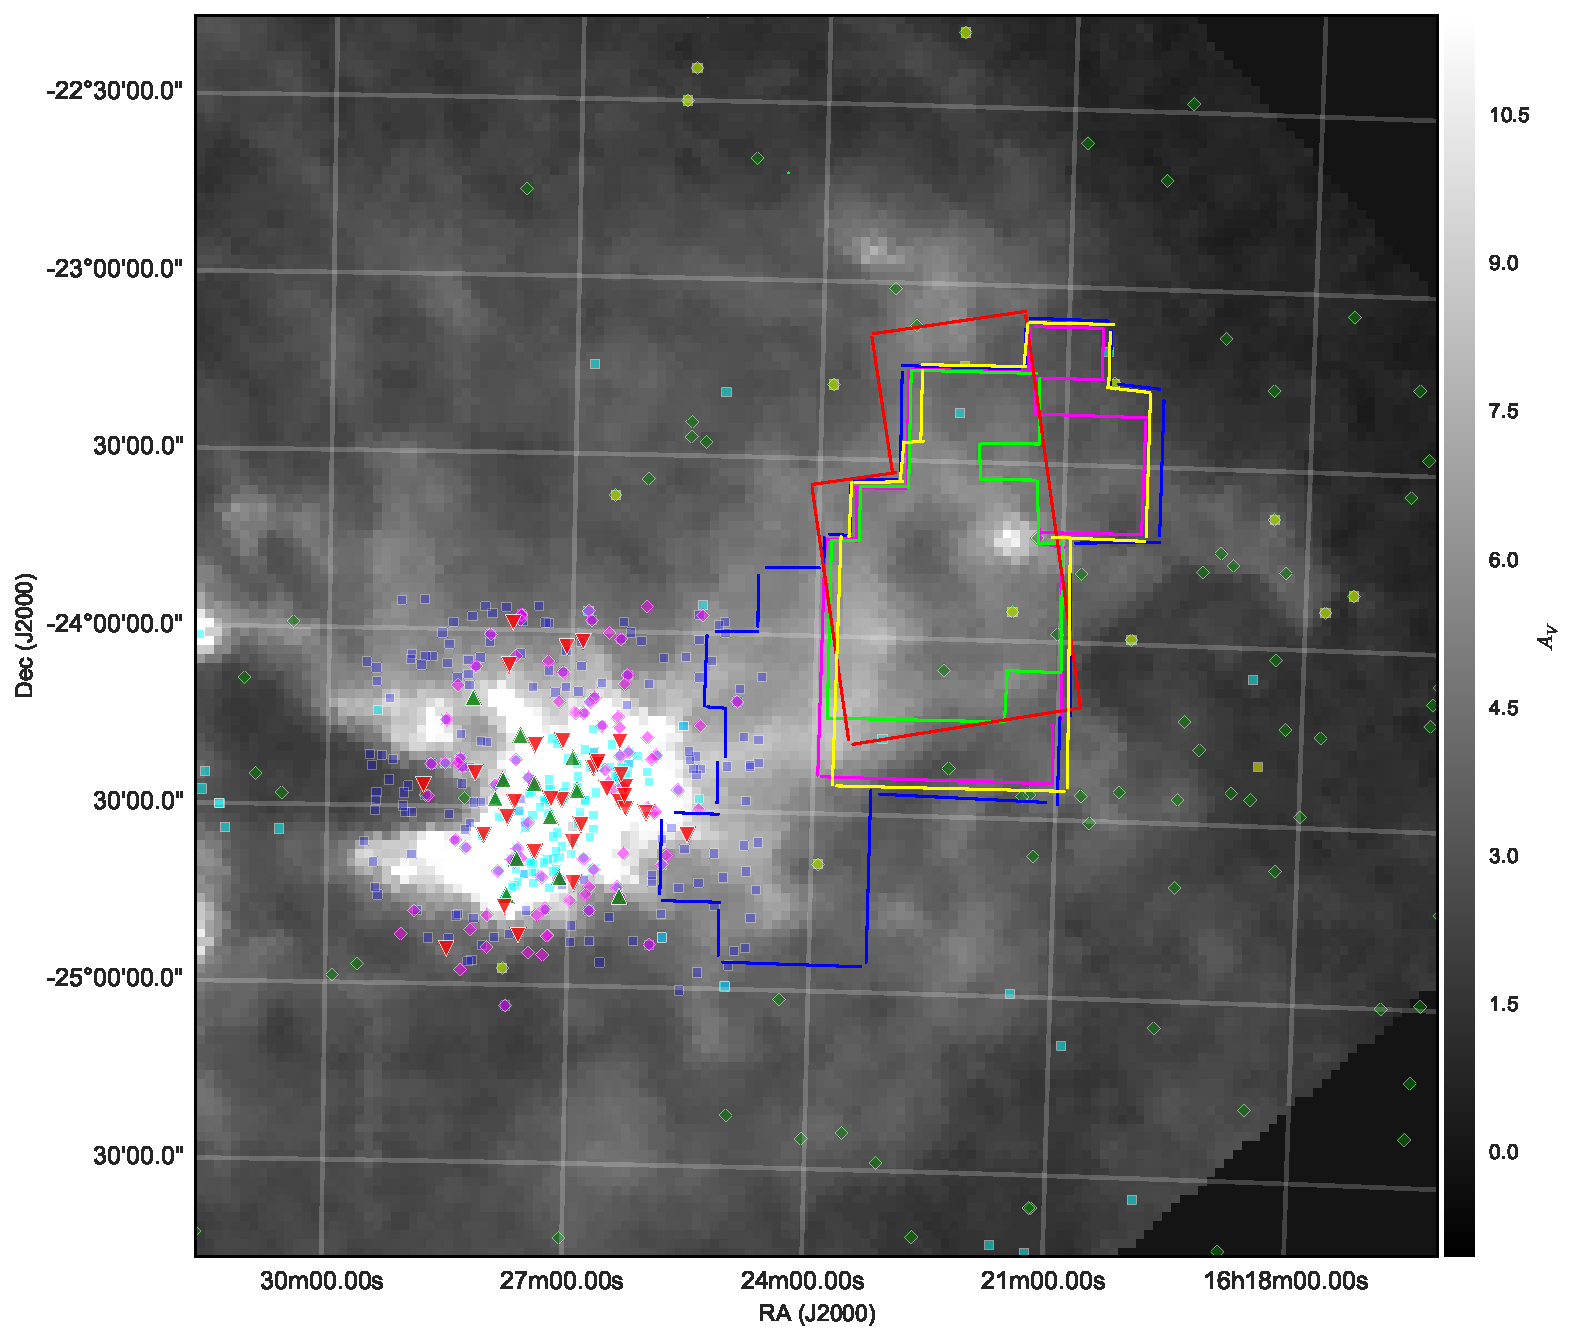
\includegraphics[scale=0.5]{chIMACS/figures/Ophiuchus_map}
\end{figure}


\subsubsection{c2deep from Harvey et al.}
We acquired a catalog of deep [5.8] and [8.0] photometry from \citet{2010ApJ...720.1374H}.  The \citet{2010ApJ...720.1374H} photometry is about 1.1$-$2.4 magnitudes deeper than c2d, which enables detection of disks of 2 Jupiter mass objects in Ophiuchus \citep{allers06}.  

\subsubsection{New: W filter}
Allers et al. (in prep) designed and implemented a custom filter centered at 1.4 $\mu$m, intermediate between the $J-$ and $H-$ atmospheric windows.  This filter is about 0.2 $\mu$m wide, cutting on near the long end of $J$ and cutting off near the short end of $H$.  This photometric band was designed to distinguish between the photospheric emission of late M and L spectral types and that of reddened early FGKM spectral types.  The broad-band IJHK colors for these disparate sources are identical, while the $W-$filter band photometry shows a deficit in M-type spectra.

One potential pitfall with the $W-$band is that this wavelength region has high and variable telluric water absorption- the same water absorption we are looking for in the photospheres of late type objects.  The extinction is problematic for two reasons.  First, the absolute transmission through the filter will be low.  Second, the variability of the telluric water absorption will manifest as shifting wavelength-dependent zero-points. To ameliorate these problems we observed from the high, dry site Mauna Kea, where the telluric water absorption is much lower than other sites.  Ideally the $W-$band photometry should be taken contemporaneously with $J-$ and $H-$ bands, in order to overcome the variability problem.  The variability is especially acute for late type young brown dwarfs that demonstrate intrinsic variability from accretion \citep{2008A&A...485..155A,2014AJ....147...82C}.

Despite the telluric absorption challenge, the $W-$ filter works- it has already been successfully applied to select brown dwarfs with over 90\% confirmation rate (K. Allers, \emph{priv. comm.}).  As a demonstration of the technique, we successfully recovered known brown dwarfs from their $W-$band photometry alone.  

One main potential advantage of the $W-$band filter is its \emph{reddening insensitivity}.  K. Allers (in prep.) derives a $Q-$parameter from $J$, $W$, $H$, band.  The $Q$ value can be tuned for particular lines of sight to mitigate the effect of reddening.  

The $W-$ band photometry in this work was observed with the University of Hawaii 88" telescope with the ULBCAM imager.  The individual photometric frames were dark subtracted, divided by a normalized flat, and median combined following the procedure of \cite{allers06}.  The ULBCAM suffered a catastrophic failure of 1 of the 4 mosaicked detectors.  The remaining 3 detectors resulted in an L-shaped tiling footprint.  The observing strategy was altered to compensate for the the L-shape, and uniform coverage was achieved.

We use the Source Extractor \citep{1996A&AS..117..393B} to perform aperture photometry on the sources in mosaicked frames.  We mitigated a large number of outlier pixels by median combining the images.

%%%%%%%%%%%%%%%%%%%%%%%%%%%%%%%%%%%%%%%%%
% TABLE - Catalog Photometry
%%%%%%%%%%%%%%%%%%%%%%%%%%%%%%%%%%%%%%%%
\begin{deluxetable}{ccccc}
\tablecolumns{5}
\tabletypesize{\footnotesize}
\tablecaption{Photometry in this study \label{tbl_photomCatalog}}
\tablewidth{0pt}
\tablehead{
\colhead{Band} &
\colhead{N 3$\sigma$ Detections} &
\colhead{10$\sigma$ mag} &
\colhead{Source} &
\colhead{Ref.} }
\startdata
	\multicolumn{5}{c}{ISPI $JH$ Catalog} \\
	\hline
	$I$  & 34467 & 23.0 & MOSAIC/CTIO 4m &  1 \\
	$J$  & 54373 & 19.4 & ISPI/CTIO &  1 \\
	$W$  & 31205 & 19.1 & ULBCAM/U. Hawaii 88" &  1 \\
	$H$  & 54373 & 18.8 & ISPI/CTIO &  1 \\
	$K$  & 20470 & 18.0 & ISPI/CTIO &  1 \\
	$[5.8] $  & 9135 & 15.7 & \emph{c2deep} &  2 \\
	$[8.0]$ & 1948 & 14.9 & \emph{c2deep} &  2 \\
	$[3.6]$  & 37423 & 16.1 & c2d &  3 \\
	$[4.5]$  & 30345 & 15.5 & c2d &  3 \\
	$[5.8]$  & 11542 & 15.7 & c2d &  3 \\
	$[8.0]$  & 2878 & 12.5 & c2d &  3 \\
	$[24]$\tablenotemark{a}  & 145 & $\sim7.9$& c2d &  3 \\
	\hline
	\multicolumn{5}{c}{2MASS $JH$ Catalog} \\
	\hline
	$I$  & 6939 & 22.9 & MOSAIC/CTIO 4m &  1 \\
	$J$  & 27208 & 16.1 & 2MASS &  4 \\
	$W$  & 11226 & 16.3 & ULBCAM/U. Hawaii 88" &  1 \\
	$H$  & 27618 & 15.3 & 2MASS &  4 \\
	$K$  & 25254 & 14.5 & 2MASS &  4 \\
	$[5.8]$  & 4891 & 15.5 & \emph{c2deep} &  2 \\
	$[8.0]$ & 2173 & 14.8 & \emph{c2deep} &  2 \\
	$[3.6]$  & 18716 & 15.3 & c2d &  3 \\
	$[4.5]$  & 18604 & 15.4 & c2d &  3 \\
	$[5.8]$  & 12859 & 13.2 & c2d &  3 \\
	$[8.0]$  & 5973 & 12.4 & c2d &  3 \\
	$[24]$\tablenotemark{a}  & 452 & $\sim7.9$& c2d &  3 \\
	
\enddata
\tablenotetext{a}{The reported depth is for 8~$\sigma$.}

\tablerefs{
(1)~\citet{allers06}
(2)~\cite{2010ApJ...720.1374H}
(3)~c2d, \cite{2009ApJS..181..321E}
(4)~2MASS, \cite{2006AJ....131.1163S}
}

\end{deluxetable}
%%%%%%%%%%%%%%%%%%%%%%%%%%%%%%%%%%%%%%%%

\subsection{Catalog I. Deep JH selected (ISPI)}
Membership to the catalog requires $5\; \sigma$ detection in both $J$ and $H$ bands.  A total of 54373 sources met this criterion, setting the length of our catalog at 54373.  We refer to this catalog as the ``Deep $JH$ Catalog'', or Catalog I.  We justified the $JH$ detection requirement because these are the bands in which young brown dwarfs peak in flux.   Sources below our 5~$\sigma$ detection limits in $J-$ and $H-$ bands would stand little chance of followup near-IR spectroscopy with existing instrumentation.  Further, sources with large $I-J$, an expectation for late-type reddened young brown dwarfs, would stand even less of a chance of optical spectroscopic followup.  The astrometric solution comes from the ISPI astrometry, which is pegged to 2MASS (see \citet{allers06} for details).  

We perform either forced photometry or catalog cross-matching on the other photometric bands described above.  In cross matching, any source within a small angular width of a $JH$ catalog member is matched to the $JH$ member.  The angular width was typically between 0.5 and 1.5", depending on the quality of the WCS solution in the imaging frames.  We do not attempt to calculate an upper limit for undetected sources.  We perform cross-matching for the $K-$band, $W-$band, and the deep $[5.8]$ and $[8.0]$ photometry.  The signal-to-noise-ratio cutoffs for those catalogs are about 5, 1, 2, and 2, respectively.  

In forced photometry, we force a measurement of the flux, in the location of a detected source.  The flux measured in this way yields many upper limits.  We performed forced photometry on c2d imaging in bands $[3.6]$, $[4.5]$, $[5.8]$, $[8.0]$, and $[24]$.  The lowest $S/N$ ratio in the forced photometry approach is 0.1.   Table \ref{tbl_photomCatalog} lists the number of $>3\sigma$ detections in each band, and the typical 10 $\sigma$ magnitude, which was computed as the median flux of sources with signal noise ratio between 9.5 and 10.7 $\sigma$.

\subsection{Catalog II. Shallow $JH$ selected (2MASS)}
We also made a shallow catalog constructed with 2MASS $JH$ photometry instead of the deeper ISPI $JH$ photometry.  This catalog had the virtue that its spatial coverage included all of the auxiliary imaging bands that extended past the ISPI imaging.  Particularly, several candidates reported in \citet{2010ApJ...720.1374H} did not appear in Catalog I since they were outside the ISPI imaging region, but inside the c2deep imaging region.

We selected all sources in 2MASS with in a region with right ascension between about 16h18m and 16h27m, and declinations between about $-25^{\circ}$ and $-23^{\circ}$.  This selection resulted in 28092 sources, which is the length of this Catalog II.  We followed the same procedure as we did above for performing either forced photometry or catalog matching.  Table \ref{tbl_photomCatalog} lists the properties for this shallow 2MASS catalog.


\subsection{Candidate selection}
%Describe in detail the wittle down of the sample: Total number of sources, number used (i.e. detect in I band or exceptions from extra region)  We need to diagram this section.  Then how slit choices were made- giving numbers of sources at each stage.

%Now we have N spectra.  Ditch M of these as too faint or clobbered.  Now have Q left over.  How do we characterize these for Teff, Halpha, sodium index.

Equipped with our photometric catalog, we were prepared to select candidates for spectroscopic followup.  The IMACS spectrograph on Magellan can measure hundreds of sources, but not tens of thousands.  We had to reduce the the number of followup sources from 54373 (deep $JH$) and 28092 (shallow $JH$) to about 300 candidates, a down-select factor of about 0.5\%.  

We first considered the sensitivity of the instrument to set the limiting magnitude for $I-$ band spectroscopic followup.  Our 10 $\sigma$ photometric depth in $I-$ band is 23.0.  We set a limit of $I=21.6$ for followup spectroscopy.  We estimated that this threshold could provide sufficient signal-to-noise ratio for at least coarse spectral classification- ``Is the source late type or not?'', though higher signal to noise or auxiliary information would be needed to assign youth and therefore membership to the source.  Only two thirds of catalog had $I-$band measurements available, due to the smaller spatial coverage of the $I-$band imaging.  Of those sources with $I-$band detections, only 38\% had $I>21.6$.  We assigned a proxy limiting magnitude of $J>17.4$ for sources with $I-$band non-detections.


We devised four physically motivated selection criteria.  Each criterion incorporated a different aspect of known or expected physics.  The criteria are broadly $IJHK$ colors, $H- [3.6]$, custom $W-$filter, and mid-IR excess.  The criteria are binary-- the candidate met the criterion or it did not.  In this section we describe the motivation and justification for the details of these four selection criteria.  In the next subsection we describe the method we used for combining the various combinations of these 4 criteria to issue an observation priority for each candidate.  Table \ref{tbl_selectionScores} summarizes the 4 four criteria.

%%%%%%%%%%%%%%%%%%%%%%%%%%%%%%%%%%%%%%%%%
% TABLE - Scores
%%%%%%%%%%%%%%%%%%%%%%%%%%%%%%%%%%%%%%%%
\begin{deluxetable}{ccccccc}
\tablecolumns{7} 
\tabletypesize{\small}
\tablecaption{Binary selection criteria \label{tbl_selectionScores}}
\tablewidth{0pt}
\tablehead{
\colhead{Score} &
\colhead{Criterion} &
\colhead{IDs} &
\colhead{$N$ meet} &
\colhead{$N$ eligible} &
\colhead{$\%$ catalog} &
\colhead{$\%$ eligible} \\}
\startdata
	8 & $I-J$, $J-H$, $J-K$ & NIR & 3680 & 34469 & 6.8 & 10.7\\
	4 & $H-[3.6]$, $K-[3.6]$ & $[3.6]$ & 23112 & 42268 & 43.5 & 54.6 \\
	2 & $W-$ band & $W$ & 1180 & 31348 & 2.2 & 3.8\\
	1 & Mid-IR excess & Disk & 1407 & 14095 & 2.6 & 10.0\\
\enddata
\tablecomments{The number of catalog members eligible to meet a criterion differs from the length of the catalog (54373) due to missing data in the form of non-detections or non-observation.}
\end{deluxetable}

\subsubsection{Near-IR photometric selection}
\label{sec_NIR_selection}

The main point of this criterion was to select sources with colors indicative of- or at least \emph{consistent} with- late M spectral types.  Known young brown dwarfs at 1 Myr have spectral types later than about M6.  The full range of colors for young brown dwarfs is not known.  Our approach was to compile examples of colors of known young brown dwarfs and design criteria that would recover these objects.  The final criterion is composed of three color cuts, and one magnitude cut.

The color cuts rely heavily on $I-$band photometry, owing to this band's discriminatory power of separating red optical colors indicative of young brown dwarfs.  Most of our deep catalog members possessed $I-$band photometry, but not all.  The lacking of $I-$band measurements for some sources was because of the limited spatial coverage of the $I-$band mosaics, not because of sensitivity limits (our $I-$ band photometry is exceptionally deep).  Because of our heavy reliance on $I-$band, sources without $I-$band photometry were ineligible to meet the near-IR photometric selection criterion.  A total of 34469 out of 54373 sources had $I-$band measurements.  This choice simply means that we preferentially directed our spectroscopic observations towards the regions where $I-$band data was available.  This cut reduced the number of sources from 100\% to 63.4\%.

As mentioned above, one of the clearest signatures of brown dwarfs is their red optical color, since optical  ($R-,I-, z-$ band $\lambda \sim  0.8 \; \mu$m) is short of the peak transmission of the cool (1600$< T <$ 2900 K, $\lambda \sim$ 1.0-2.0 $\mu$m) substellar photospheres of brown dwarfs.  However the large optical minus infrared color is a hallmark of both brown dwarfs and high-$z$ galaxies, and can be mimicked by the effect of high reddening.  The $I-J$ color of brown dwarfs with spectral types later than $\sim$M7 is typically greater than $\sim2.85$ \cite{allers06}.  Reddening would only act to make this value larger.  So we required $I-J +\sigma_{I-J} > 2.85$, where $\sigma{I-J}$ is the measurement uncertainty of $I-$ and $J-$ bands added in quadrature.  This $I-J$ color cut was met by 12548/54373 ($23.1\%$) of the total catalog members, or 12548/34469 (35.4\%) of those sources possessing $I-$band measurements. 

Our next color cut is to select for blue intrinsic $J-H$ colors.  All sources in our catalog have detections in $J-H$. The motivation for this color cut is that observed young brown dwarfs demonstrate a relatively tight range in intrinsic $J-H$ (typically 0.58-0.71 for M5-M9), so we could eliminate contamination by setting the threshold redward of the largest $J-H$ we could expect.  We set that threshold at 0.84156, on the MKO scale.  A large extinction could pull the observed value past the 0.84156 threshold.  So we constructed a reddening line that related the observed $I-J$ with the observed $J-H$ through the selective extinction ratios $A(\lambda)/A_V$ compiled from ADPS \citep{2000A&AS..147..361M} with $R_V=3.1$.  The color cut is: $I-J + \sigma_{I-J} > 2.85 + [(J-H) - 0.84156 + \sigma_{J-H}]\frac{A_I-A_J}{A_J - A_H}$.  Where $\sigma_{I-J}$ is the uncertainty in the $I-$ and $J-$ bands added in quadrature, and $\sigma_{J-H}$ is the uncertainty in $J-H$ added in quadrature.  The ratio $\frac{A_I-A_J}{A_J - A_H}$ is equal to 3.33, and takes into account the selective extinction.  Figure \ref{fig_NIR_selection_JH} shows this color cut as the diagonal line.  The upper left portion of the plot meets both color cuts discussed so far.  The upper right corner has red $I-J$ color, but has $J-H$ color that is too red for an M9 to be explained by reddening alone.  This color cut alone was met by 8105/54373 sources (14.9\%).  At this point, 3967 sources (7.3\% of the catalog) met all the previous color cuts.

\begin{figure}[ht!]
  \caption{Color-color cuts in $I-J$ vs $J-H$. The horizontal dashed line shows $I-J=2.85$.  The tilted dotted line demonstrates the selection for intrinsic blue $J-H$ colors ($<0.84156$), allowing for reddening.  The grayscale Hess diagram in the background shows the density of points in each color bin, constructed from 34469 sources with $I-$band detections.  The points in the upper left quadrant of the diagram meet the color cuts 2 and 3 from the list in Section \ref{sec_NIR_selection}.  The magenta circles are sources from \citet{allers06} that have spectral types between M6 and L2 \citep{2011ASPC..448..633G}.\label{fig_NIR_selection_JH}}
\centering
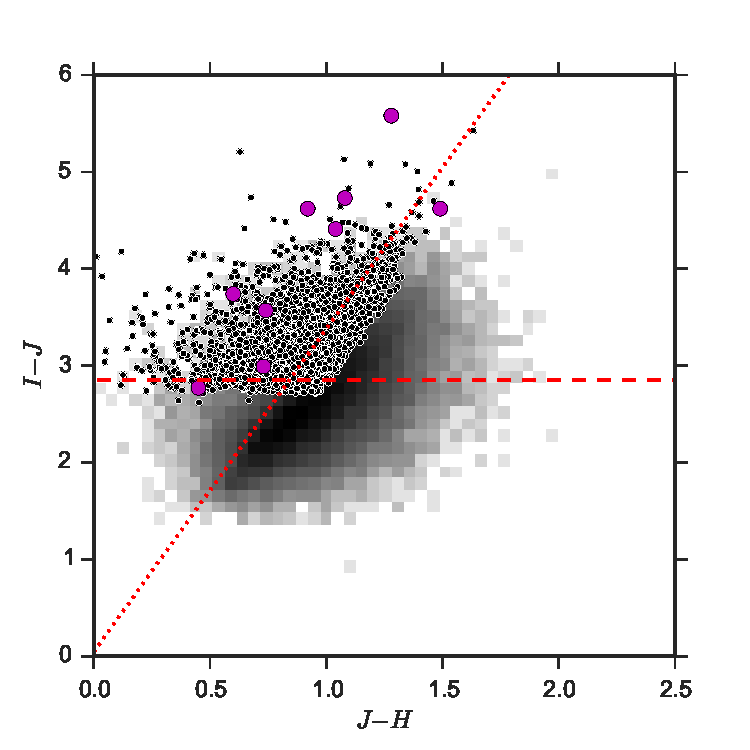
\includegraphics[scale=0.6]{chIMACS/figures/NIR_selection_allers_M6_L2}
\end{figure}

We leveraged the $K-$band photometry when it was available to make another color cut.  Like the $I-$band data, the $K-$ band had incomplete spatial coverage-- only 38\% of sources had a $K-$band measurement available.  Our strategy here was similar to the color cut above selecting for blue intrinsic $J-H$ color, except now we are selecting for intrinsic blue $J-K$ color.  We assumed a maximum $J-K$ for brown dwarfs of 1.37662 in the MKO system.  We then built a reddening relationship between $I-J$ and $J-K$ that takes into account the selective extinction in from ADPS, as above.  Lastly, we removed sources that were redder than this curve, removing only sources that had $K-$band available.  The sources we removed satisfied this criterion:  $I-J + \sigma_{I-J} < 2.85 + [(J-K) - (J-K)_0 - \sigma_{J-K}]\frac{A_I-A_J}{A_J - A_K}$, where $\sigma_{I-J}$ is the same as it is above, and $\sigma_{J-K}$ is the photometric measurement uncertainty in $J-$ and $K-$ bands added in quadrature.  This color cut was met by 11020/54373 sources, which means that the complement, or 43353 passed on.  Combining this criterion with the previous color cuts brings the passage rate from 7.3\% from the previous cuts to 6.8\% including this one.

\begin{figure}[ht!]
  \caption{Color-color cuts in $I-J$ vs $J-K$. The horizontal dashed line shows $I-J=2.85$.  The tilted dotted line demonstrates the selection for intrinsic blue $J-K$ colors ($<1.37662$), allowing for reddening.  The grayscale Hess diagram in the background shows the density of points in each color bin, constructed from 19733 sources with both $I-$ and $K-$band detections.  The points in the upper left quadrant of the diagram meet the color cuts 2 and 4 from the list in Section \ref{sec_NIR_selection}.  The square boxes plotted are sources from \citet{allers06} which have spectral types between M6 and L2 \citep{2011ASPC..448..633G}.\label{fig_NIR_selection_JK}}
\centering
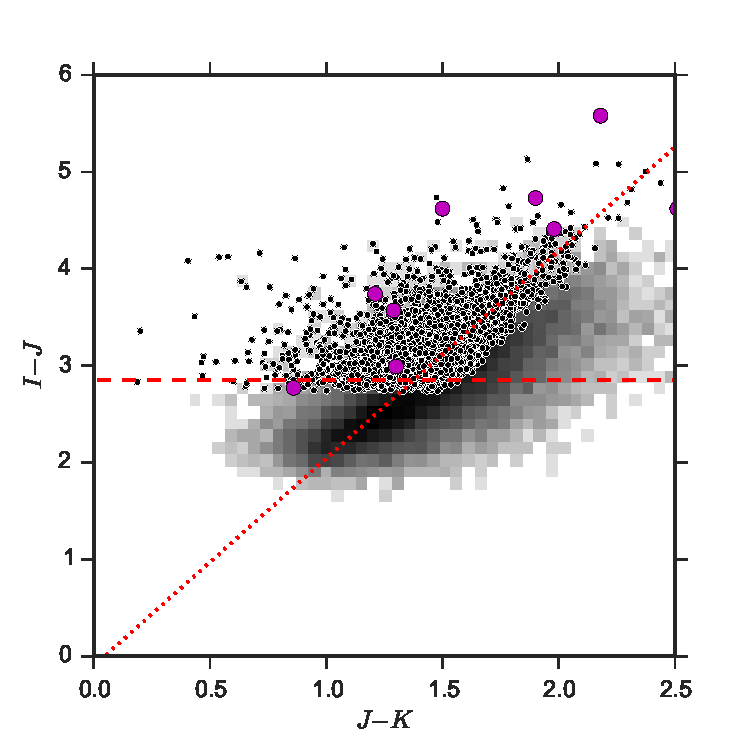
\includegraphics[scale=0.6]{chIMACS/figures/NIR_selection_JK_allers_M6_L2}
\end{figure}


Lastly, we applied a $K-$ magnitude cut, with the intention of finding the faintest and therefore lowest luminosity young brown dwarfs.  For a given cluster age, the lowest luminosity young brown dwarfs are also likely to be the lowest mass.  We deemed these lowest mass sources to be most scientifically interesting.  Following \citet{allers06}, we assumed an absolute $K-$band magnitude of 8.01 for a young M9, and a distance modulus $\mu=5.48$, for a $K-$band apparent magnitude cut of $K + \sigma_{K} > 13.49$, where $\sigma_K$ is the photometric measurement uncertainty in the $K-$band.  Since $K-$band data was unavailable for many sources, we also removed sources consistent with $H-$band apparent magnitudes less than 8.51 plus the distance modulus, keeping sources with: $H+\sigma_{H} > 13.99$.  Again, we sought sources fainter than this limit since we were most interested in low luminosity, low mass brown dwarfs.  This criterion is likely to cut sources with spectral types earlier than M9.  This magnitude cut was met by 1105 sources out of the 54373 source catalog.  When combined with the previous color cuts above, this magnitude cut removed 14 sources: OPH\_675, OPH\_672, OPH\_679, OPH\_678, OPH\_673, OPH\_674, OPH\_12081, OPH\_12079, OPH\_3054, OPH\_5413, OPH\_12961, OPH\_13049, OPH\_19613, and OPH\_956.

\begin{figure}[ht!]
  \caption{$H-$band Magnitude cut.  The horizontal dashed line shows $H=13.99$.  The grayscale Hess diagram in the background shows the density of points in each color-magnitude bin, constructed from the entire 54373 point ISPI deep $JH$ source catalog.  The circles are sources from \citet{allers06} towards \emph{Ophiuchus}.  The two \citet{allers06} sources with $H>13.99$ have M8 spectral types, while th others are M6 or earlier \citep{2011ASPC..448..633G}. \label{fig_NIR_selection_H}}
\centering
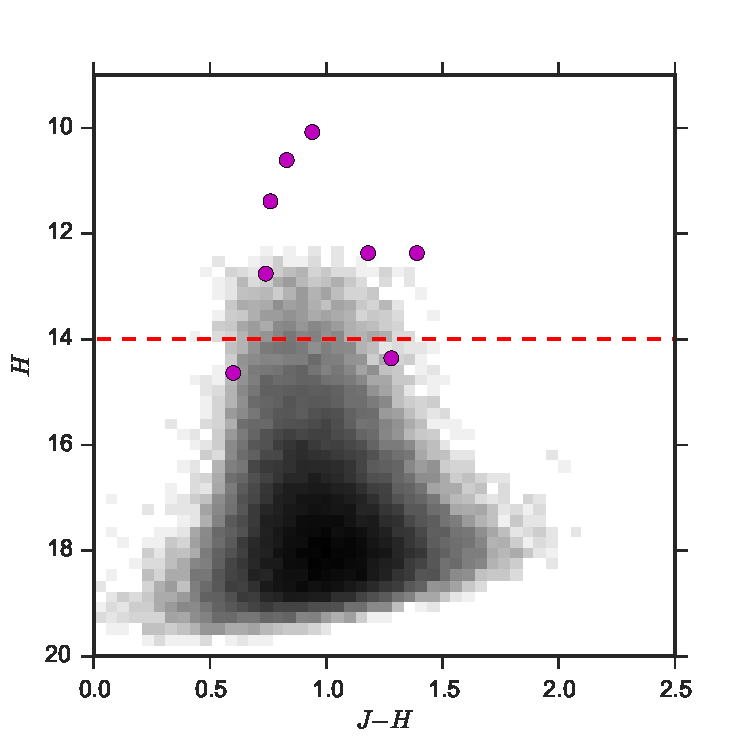
\includegraphics[scale=0.6]{chIMACS/figures/NIR_selection_H_allers_oph}
\end{figure}


To summarize, our near-IR selection criterion is composed of the union of all of these color and magnitudes cuts:
\begin{enumerate}
\item $I-$band detection
\item $I-J +\sigma_{I-J} > 2.85$
\item $I-J +\sigma_{I-J} > 2.85 + (A_I-A_J)  \times ((J-H) - (J-H)_0)/ (A_J - A_H)$
\item When $K-$band is available: $I-J + \sigma_{I-J} > 2.85 + [(J-K) - (J-K)_0 - \sigma_{J-K}]\frac{A_I-A_J}{A_J - A_K}$ 
\item $K + \sigma_{K} > 13.49$ or  $H+\sigma_{H} > 13.99$
\end{enumerate}


\subsubsection{Mid-IR excess (disk) selection criterion}
\label{sec_midIR_selection}
Sources detected at 24 $\mu$m with greater than 3 $\sigma$ confidence were automatically considered disk sources, since we assumed $[24]$ could not detect photospheric emission for our low luminosity sources.  The 3 $\sigma$ depth for 24 $\mu$m is $\sim~$9.8 magnitudes, so given the assumed distance modulus to \emph{Ophiuchus} of 5.48, the absolute magnitude of the photosphere would have to be 4.3, which is brighter than we expect for young brown dwarfs without disks.  Only 200 sources had $>3\;\sigma$ detection at $[24]$.

We required a $2\;\sigma$ detection in $[3.6]$ and a $2\;\sigma$ detection in any one of $[5.8]$, $[8.0]$, or $[24]$.  Only 14095 sources met this cut.  

Sources had to demonstrate a 2 $\sigma$  excess above both the photospheric $[3.6]-[5.8]$ color and $[3.6]-[8.0]$ color.  We defined the photospheric mid-IR colors of $[3.6]-[5.8]=0.08$ and $[3.6]-[8.0]=0.21$ \citep{2006ApJ...651..502P}.  Figure \ref{fig_midIR_selection} shows this color cut.  In total, 1558 sources met this color cut.  

Note that the mid-IR excess threshold as defined above is fairly liberal- sources marginally above the assumed photospheric emission threshold would be counted as mid-IR excess.  This minuscule degree of excess could be consistent with no disk whatsoever and unusually red mid-IR colors.  Our choice to set this liberal threshold was that the deep \emph{Spitzer} imaging could detect exceptionally weak mid-IR excess.  We would expect diskless young sources to be clustered around the intersection of the dashed and dotted lines in Figure \ref{fig_midIR_selection}.  \emph{Anemic} disks would occupy the region of color-color space between the diskless sources and the colored circles representing the \citet{allers06} sources.  All-together 1407 sources met all of the above criteria consistent with mid-IR excess.


\begin{figure}[ht!]
  \caption{$[3.6]-[5.8]$ vs $[3.6]-[8.0]$ color plot, demonstrating the mid-IR excess selection criterion.  The grayscale Hess diagram shows the density of 14095 sources in our sample possessing a 2 $\sigma$ detection in $[3.6]$ and a 2$\sigma$ detection in at least one of $[5.8]$, $[8.0]$, or $[24]$.  The horizontal dashed line is $[3.6]-[8.0]=0.21$, the vertical line is $[3.6]-[8.0]=0.08$ \citep{2006ApJ...651..502P}.  Sources meeting the criteria described in Section \ref{sec_midIR_selection} are primarily in the upper right quadrant.  Some sources with 3$\sigma$ $[24]$ detections are in the other quadrants.  The large colored circles are all sources from \citet{allers06}. \label{fig_midIR_selection}}
\centering
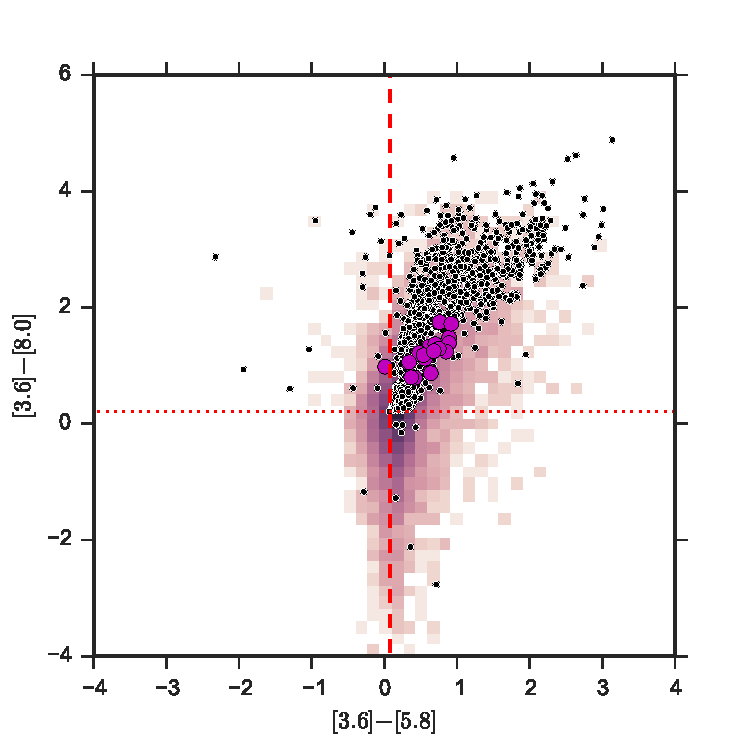
\includegraphics[scale=0.6]{chIMACS/figures/disk_selection_allers}
\end{figure}

\subsubsection{$W-$ filter selection criterion}
The $W-$filter is a custom near-IR filter (Allers et al. \emph{in prep.}).The $W-$ filter works because the photospheres of cool stars and brown dwarfs have intrinsic water absorption.  The degree of water absorption depends on the temperature of the emission region, which we approximate as the effective temperature $T_{\mathrm{eff}}$.  We  quantified the degree of intrinsic water absorption with a $Q$ parameter from the trio of $J-$, $W-$, and $H-$ magnitudes (Allers et al. \emph{in prep.}).  The $Q$ parameter is zero for no evidence of water absorption, and negative when water absorption is present.  The water absorption is stronger for cooler photospheres- M6 has a $Q$ value of about -0.5, and L0 has a $Q$ value of about -1.0.  

A total of 31348 sources (57.6\% of the catalog) had $W-$band photometry.  Since all sources in our catalog had $J-$ and $H-$ band photometry, all 31348 sources with a $W-$band measurement were issued a $Q$ value.  Figure \ref{fig_Q_value_histogram} shows the histogram of the $Q$ values.

We designed our $W-$band selection criterion around the value of the $Q$ parameter. Sources met the $W-$band criterion if they were within the boundary $-0.5<Q<-2.5$.  We required a 2 $\sigma$ measurement of $Q$ inside those bounds, where $\sigma$ is the uncertainty in the $Q$ value propagated from the photometric and calibration uncertainties in the $W-$band.  A total of 1180 sources met the $W-$filter selection criterion.  The number 1180 is 2.1\% of the entire catalog, or 3.7\% of those sources possessing a $W-$band detection.  Figure \ref{fig_Q_value_histogram} shows the selection boundaries as vertical lines in the histogram, with the fraction of sources meeting the criterion highlighted in a different shade.  Based on preliminary trials of the $W-$ filter, we expected this range in $Q$ values to correspond to M8 spectral types.

\begin{figure}[ht!]
	\caption{Histogram of the $Q$ value derived from $W-$band photometry.  The vertical dashed lines represent the boundaries of the selection method.  The dark colored region region interior to the boundaries indicates the 4\% of sources detected in $W-$band meeting our selection criteria.  \label{fig_Q_value_histogram}}
\centering
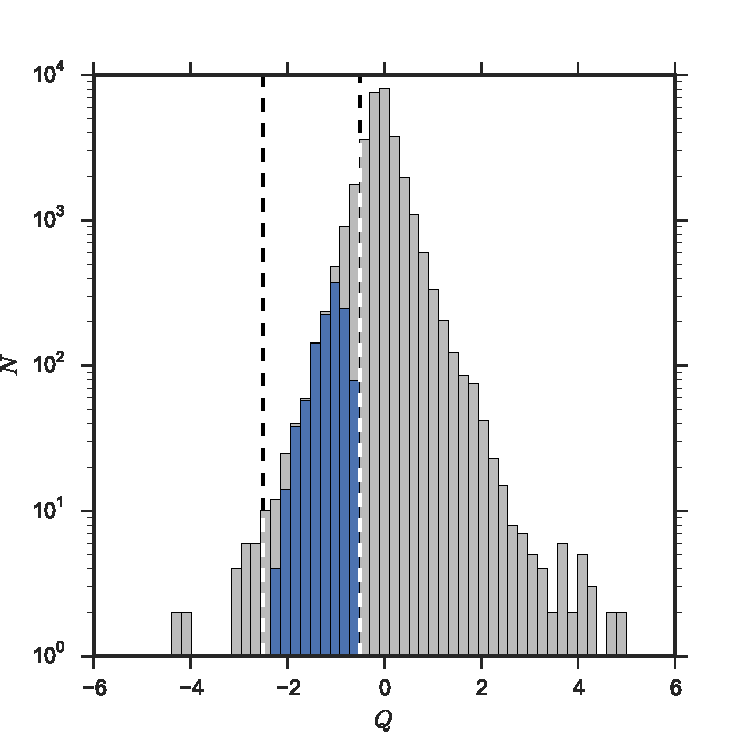
\includegraphics[scale=0.6]{chIMACS/figures/W_phot_sel_mgs}
\end{figure}

\subsubsection{$H-[3.6]$ color selection criterion}
We required the $H-[3.6]$ color to appear redward of the assumed photospheric colors.  We assumed photospheric colors from \citet{2006ApJ...651..502P}.  The motivation for this color cut was that extinction and mid-IR excess emission both act to increase $H-[3.6]$.  In principle $[3.6]$ can exhibit finite disk excess, as is seen in $T-Tauri$ stars.  However, we expect brown dwarfs to exhibit negligible excess at $[3.6]$, based on radiative transfer models that show brown dwarf mid-IR excess detaches from the photosphere at wavelengths $>4$ micron \citep{2009MNRAS.394L.141E}.  Our selection criterion required a $[3.6]$ measurement, albeit at any signal-to-noise ratio.  We required $H-[3.6] + \sigma > 0.8$, where $\sigma$ is the photometric measurement uncertainty in $H-$ and $[3.6]$ bands added in quadrature.  For objects with existing $K-$ band photometry we further required $K-[3.6] - \sigma > 0.49$, where $\sigma$ is the photometric measurement uncertainty in $K-$ and $[3.6]$ bands added in quadrature.  All combined, 23112/54373 sources passed this criterion.  Note that we did not apply a signal-to-noise ratio cut on $[3.6]$, which is evinced in Figure \ref{fig_midIR_phot_sel}- sources with large measurement uncertainty still meet our criterion.  Notice also that the $K-[3.6]$ color cut is more stringent than the $H-[3.6]$ color cut; the $K-[3.6]$ demands a 1$\sigma$ excess over 0.49, whereas the $H-[3.6]$ can be merely consistent with 0.8.

\begin{figure}[ht!]
  \caption{$H-[3.6]$ color criterion.  The gray histrogram shows the distribution of the 42268 sources in the catalog with a $[3.6]$ measurement, while the colored histogram shows the distribution of sources with $H-[3.6]$ consistent with being in excess of the photospheres of young brown dwarfs, shown as the vertical line at 0.8.\label{fig_midIR_phot_sel}}
\centering
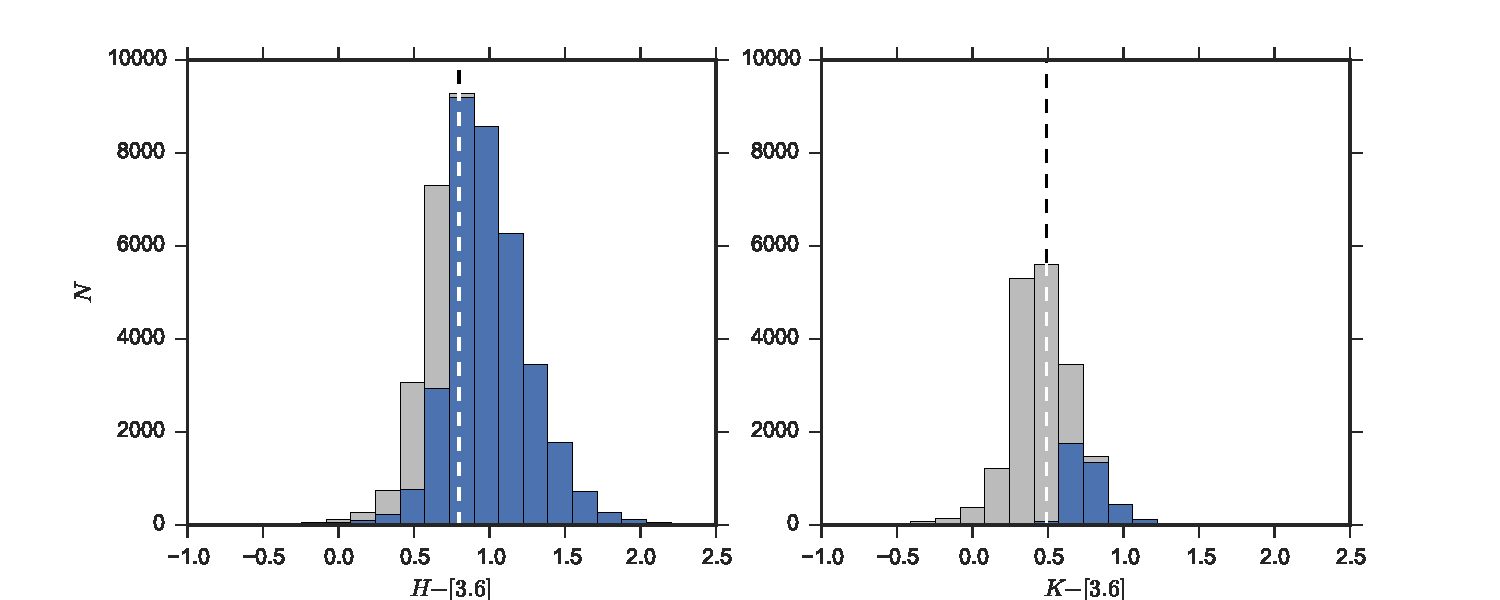
\includegraphics[scale=0.6]{chIMACS/figures/midIR_phot_sel}
\end{figure}



\subsection{Ranking the combinations of selection criteria}
Table \ref{tbl_scoring2Priority} shows our scoring system for translating selection criteria into priority for observation.  Naturally, the candidates that met all criteria were ranked as the highest priority for observations, since we deemed these sources as most likely to be spectroscopically confirmed as young brown dwarfs.  Sources that met none of our four criteria were dismissed.  Sources that met some of the criteria but not others were rank ordered based on the tradeoff for what was most likely to pan out, and what was most scientifically interesting.  We kept the top ten priorities.


%%%%%%%%%%%%%%%%%%%%%%%%%%%%%%%%%%%%%%%%%
% TABLE - Scoring to Priority conversion
%%%%%%%%%%%%%%%%%%%%%%%%%%%%%%%%%%%%%%%%
\begin{deluxetable}{cccccc}
\tablecolumns{6} 
%\tabletypesize{\footnotesize}
\tablecaption{Selection-priority scoring system\label{tbl_scoring2Priority} } 
\tablewidth{0pt}
\tablehead{
\colhead{Priority} &
\colhead{Scores} &
\colhead{Net Score} &
\colhead{IDs} & 
\colhead{$N$ $I<21.6$} &
\colhead{$N$ $I>21.6$} }
\startdata
1	 & 1,2,4,8 &15 & Disk, $W$, [3.6], NIR & 7 & 5 \\
2	 & 2,4,8 &14 & $W$, [3.6], NIR & 27 & 138 \\
3	 & 1,4,8 & 13 & Disk, [3.6], NIR & 17 & 30 \\
4	 & 1,2,8 & 11 & Disk, $W$, NIR & 1 & 0 \\
5	 & 1,2,4 & 7 & Disk, $W$, [3.6] & 15 & 12 \\
6	 & 1,2 & 3 & Disk, $W$ & 10 & 5 \\
7	 & 2,8 & 10 & $W$, NIR & 11 & 109 \\
8	 & 1,8 & 9 & Disk, NIR & 10 & 20 \\
9	 & 2,4 & 6 & $W$, [3.6] & 103 & 158 \\
10 & 2 & 2 & $W$ & 282 & 297 \\
other & - & - & - & \multirow{2}{*}{53116} \\
\enddata
\end{deluxetable}


Here we briefly justify our rankings for the second and third place priority rankings.  The prospect of discovering diskless young brown dwarfs directly addressed our science question of whether disks around young brown dwarfs are longer lived than their T-Tauri counterparts \citep{2008ApJ...681.1584R}.  So sources that met all criteria except the mid infrared excess criterion were ranked priority 2.  These sources, if confirmed, represent Class III analogs to T-Tauri stars.  Priority 2 sources are also consistent with foreground or background M or L type dwarfs, so we projected high levels of contamination.

Priority 3 sources are analogous to most other surveys for young brown dwarfs.  Specifically, priority 3 sources meet all three of our conventional broad band photometric criteria, but they do not meet our custom $W-$ criterion.  Table \ref{tbl_scoring2Priority} summarizes the rest of the priorities.


\subsection{Whittling down from 54373 to $\sim$500}
Equipped with a prioritized list of candidates, we designed multi-object slit masks for IMACS \citep{2011PASP..123..288D}.  The MaskGen software\footnote{See \url{ http://code.obs.carnegiescience.edu/maskgen}} takes a prioritized list of sources and optimizes the placement of slits for the highest scientific return.  Our science goal required a wavelength range of $\sim 650-900$ nm for broad-band spectral typing and H$\alpha$ equivalent width measurement.  Measurement spectrally narrow gravity-sensitive features indicative of youth \citep{1999ApJ...525..466L,2007AJ....134.2398C,2009AJ....137.3345C} was top level requirement.  This requirement imposed required spectral resolution $\sim1000$.  These specifications limited the number of slits that fit on a multi-object slit mask to $\sim100$.

The IMACS $F/2$ camera delivers a $27.4'$ diameter field of view.  It would take six such IMACS fields to cover the spatial extent of our entire catalog.  We made 6 slit masks in total.  Availability of bright Shack-Hartmann stars limited the available center positions and rotations of the masks.  We settled on center positions that included the most priority 1's, 2's, and 3's.  The center positions, orientation, and slit positions of all the slit masks are downloadable online \footnote{\url{http://www.lco.cl/telescopes-information/magellan/instruments/imacs/making-and-submitting-imacs-slitmasks}}.  Table \ref{tbl_IMACSslitMasks} lists the slit masks used in this study.  More details of the slit masks can be found at the IMACS slitmask archive.

%%%%%%%%%%%%%%%%%%%%%%%%%%%%%%%%%%%%%%%%%
% TABLE - Slit mask properties
%%%%%%%%%%%%%%%%%%%%%%%%%%%%%%%%%%%%%%%%
\begin{deluxetable}{cccccc}
\tablecolumns{6} 
\tablecaption{IMACS $F/2$ multi-object slit masks \label{tbl_IMACSslitMasks}}
\tablewidth{0pt}
\tablehead{
\colhead{Name} &
\colhead{$N$ slits} &
\colhead{Obs. Dates} &
\colhead{Net Exp. time} &
\colhead{Filter} & 
\colhead{Center RA \& Dec.} \\
\colhead{-} &
\colhead{\#} &
\colhead{YYYYMMDD} &
\colhead{hours} &
\colhead{-} &
\colhead{J2000}}
\startdata
	nc200\_75 & 76 &  20100617 & 2.50  & spectroscopic-2 & 16:21:25 -23:26:42.5\\
	southwes & 72 & 20100617 & 2.00  & spectrosopic-2 & 16:21:44.8 -24:08:45.5\\
	southeas & 45 & 20110707 & 2.25  & 5694-9819 & 16:22:36 -23:54:27 \\
	nc\_2011 & 104 & 20110707 & 4.66 &  5694-9819 & 16:21:25 -23:26:42.5 \\
	sw\_2011 & 101 & 20120513 & 3.58  & WB6300-9500 & 16:21:44.8 -24:08:45.5 \\
	ophwes & 25 & 20120513 & 0.76  & WB6300-9500 & 16:21:29.3 -23:48:38.2 \\
	ophne & 107 & 20120513, 20120514 &  4.38 & WB6300-9500 & 16:21:58.1 -23:17:54.7\\
\enddata
%\tablecomments{The spectroscopic-2 filter has $>80$\% transmission from 3700 $\angstrom$ to 10000 $\angstrom$. The 5694-9819 filter has wavelength range 5694$-$9819 $\angstrom$.  The WB6300-9500 filter has wavelength range 6300$-$9500 $\angstrom$. }
\end{deluxetable}

%------------------------------------------------------------------------------------------
\section{Spectroscopic observations}
%------------------------------------------------------------------------------------------

\subsection{IMACS observations}
\subsubsection{Observing Dates and conditions}
In this section we describe the observations.  We acquired 530 spectra on six different slitmasks over three years.  Table \ref{tbl_IMACSslitMasks} lists the observation dates and on-sky exposure time for all six of the masks.

\subsubsection{Instrumental setup- special note on filters}
We computed spectral response corrections by observing relatively featureless A0V stars and White Dwarfs.  We normalized the spectra for the observed White Dwarfs LTT7987 and LTT3218 by their counterpart model spectra from \citet{2014A&A...568A...9M}.  The A0V stars were normalized by a synthetic model.  The normalized spectral response correction is dominated by a smoothly varying component (filters, grating blaze, etc) and sharp features (telluric atmosphere).  We manually corrected spectral artifacts surrounding $H\alpha$.

We used three different filters, not all at the same time- ``Spectroscopic 2'', ``5694-9819'', and ``WB6300-9500''.  The ``Spectroscopic 2'' filter had a short wavelength cutoff $<4000 \angstrom$, which resulted in second order overlap for wavelengths longer than $8000 \angstrom$.  For our intrinsically red sources this choice does not affect the spectra.  However, the telluric A0V and White Dwarf calibrators are very blue, causing strong second order overlap.  For the observations with this filter we generated a synthetic spectral response correction.  We computed an average spectral response from the 2012 observing season, observed through the ``WB6300-9500'' filter.  We divided out the published filter response and multiplied back by the Spectroscopic-2 filter curve.  We then applied this synthetic spectral response to the affected 2010 and 2011 spectra.

\subsection{IMACS Multi-slit exposure 2D spectral extraction}
\subsubsection{Cosmos 2-16}
We reduced all of the multi-object spectroscopy with the facility data reduction package \texttt{Cosmos}\footnote{See \url{http://code.obs.carnegiescience.edu/cosmos}} \citep{2011PASP..123..288D} , which includes an algorithm for optimal sky subtraction \citep{2003PASP..115..688K}.  We used \texttt{Cosmos} version 2-16.  \texttt{Cosmos} maps each spectrum from the multi-slit exposure, beginning with the coarse optics model of the instrument.  \texttt{Cosmos} iteratively refines the mapping solution to produce flat-fielded, sky-subtracted, rectified, 2D spectra for each slit.  We wrote custom IDL scripts\footnote{All of the code used for this paper is available on GitHub: \url{https://github.com/BrownDwarf/BAADE}} to automatically run through the \texttt{Cosmos} cookbook for all of the multi-slit exposures.  Mapping solutions should be accurate to one-tenth of a pixel \citep{2011PASP..123..288D}, we found mapping solutions were typically $<0.3$ pixels, and as high as 1-3 pixels for the bottom $10\%$ of slit fits.  The long tail outliers arise when secondary images overlapped the arc lamp spectra in the multi-slit exposures.  The secondary images were bright zero-order slit images, or second-order spectra.


All spectra went through a coarse spectral extraction which determined the average center position and tilt of the spectral traces.  The traces for the lowest signal-to-noise-ratio sources were unreliable, and were simply replaced with the mean center position for the high signal-to-noise-ratio traces.  The width extraction width was increased to safely capture the unknown trace position.  The spectra were then re-extracted with the revised estimate for the center position and width.

\subsubsection{Problem with 2010 clobbering}
The \texttt{Cosmos} spectral mapping step was especially problematic for mask nc200\_75 due to slit overcrowding- spectral traces overlapped.  Particularly the ``extend\_slits'' feature caused many spectral traces to lose $\sim50$ nm chunks of spectra from overlapping zero order images.  The overcrowding also interfered with the arc-lamp calibration frames, since zero and second order images over-crowded the spectral traces.  These artifacts flowed down to poor spectral mapping, which flowed down to poor sky subtraction and deformed traces in the 2D spectrum.  The ``extend\_slits'' option was disabled in all future slit masks, which dramatically reduced zero- and second- order images, resulting in much better spectral mapping and wavelength calibration.  Still, the nc200\_75 slit masks show acceptable performance in the spectral regions that survived.  Most of the artifacts were simply masked out.

\subsection{Spectral reduction}

\subsubsection{Overall strategy}
Equipped with rectified 2D spectra, we extracted 1D spectra with conventional methods and some custom IDL routines.  Our custom routines automatically riffled through all multi-slit exposures to reduce user intervention and enhance repeatability for the hundreds of individual spectra.  The main challenge was to automatically identify low signal to noise ratio traces or handle traces distorted from poor 2D mapping.  The spectral trace delivered by the \texttt{Cosmos} 2D spectral mapping is characterized by the pixel position of the center, and a rotation from the pixel $x-y$ basis.  The lowest signal to noise ratio traces were assigned the average center positions and rotations of the brightest traces, which worked fairly well at matching the visually identified traces for low signal to noise ratio spectra.  The low signal to noise ratio spectra were ultimately not useful for purposes beyond coarse spectral classification anyways.

\subsubsection{Telluric correction}
We observed B type stellar spectral standards to correct for instrument response and telluric absorption.  We placed the telluric standard in one of the slits on a slit mask, rather than switching masks to a long-slit.  This practice resulted in some zero-order overlap around 7250 $\angstrom$ for the NC200\_75 slit mask.  We observed both A0V stars and white dwarfs.  For A0V stars we estimated the ``True'' signal as a black body of temperature equal to the effective temperature for the spectral type of the telluric standard \citep{2000asqu.book.....C}.  We observed LTT7897, and LTT3218, white dwarfs with detailed model spectra available \citep{2014A&A...568A...9M}.  We achieved the best quality telluric corrections from the white dwarf stars, so we mostly used these when available.  We did not smooth the spectral response, which adds some variance noise to our results.  However the signal-to-noise ratio in the telluric reference spectra are so high that this additional noise is negligible.

\subsubsection{Performance of spectral type standards compared to literature}
We observed several spectral type standards to demonstrate that we can reproduce the observed spectra of known late type sources.  Specifically, we observed an L2 dwarf, 2MASS J11553952-3727350 \citep{2008AJ....136.1290R}; an M9 dwarf, 2MASS J15101685-0241078 \citep{2008AJ....136.1290R}; an L0pec, J00100009-2031122 \citep{2007AJ....133..439C}; and two young M7.75 members of Chamaeleon I, ChaH$\alpha$1 and ChaH$\alpha$7 \citep{2004ApJ...602..816L}.  We overplotted our spectra with published spectra to compare and contrast.  The spectra showed overall agreement in their spectral shapes.  The main differences were that some of the published spectra were not telluric corrected so the telluric band at 7600 \angstrom appears in excess in our spectra.  The spectra from the NC200\_75 slit mask exhibit an artifact at 7250 \angstrom, as mentioned above.  Since this artifact is attributable only to the particular choice of this slitlet, most spectra from this mask will not have an artifact in the same location, though the presence of artifacts in the NC200\_75 slit mask was relatively common.

Single pixel defects were also conspicuous in our comparison spectra.  These defects are mostly uncorrected cosmic rays.  They are most prominent in the spectra of low signal-to-noise ratio spectra, and are about 10 to 20 times the typical pixel-to-pixel variance.  It is easy to identify these as cosmic rays during visual comparison.  However, automated spectral analysis like equivalent width measurements and continuum estimation can be affected by these large outliers.  We employ robust algorithms (\emph{e.g.} median instead of mean) when available, and manually flag pixels when needed.

Based on the excellent accord in our spectra and published spectra, we would expect to derive identical spectral types to the published ones.  We are therefore confident in all of the spectral response corrections and extraction strategies applied to our spectra, and deem their spectral slopes as trustworthy, inasmuch as the published spectra are too.


%------------------------------------------------------------------------------------------
\section{Spectral and photometric analysis}
%------------------------------------------------------------------------------------------

\subsection{Spectral classification with \emph{The Hammer}}
We visually inspected the spectra for evidence of broad-band molecular absorption in the IMACS $I-$band spectra in the region $6500<\lambda(\angstrom)<9000 $.  The broad FeH, VO, and TiO bands are characteristic of late M spectral types, and are conspicuous even in smoothed low signal-to-noise ratio spectra.  To accelerate the process of visually classifying hundreds of spectra, we employed Version 1.2.5 of \emph{The Hammer} spectral typing code \citep{2007AJ....134.2398C,2011AJ....141...97W}.  \emph{The Hammer} first computes a machine spectral type based on several spectral type sensitive indices.  Then \emph{The Hammer} overlays user-selectable comparison spectra, which can be visually matched to the overall spectral shape.  \emph{The Hammer} does not have a mechanism for tuning the extent of wavelength-dependent extinction, so we anticipate that matches to the observed spectra will lead us to overestimate the spectral type.  That is we will derive spectral types later, by 1-3 spectral subtypes, than we would have if we knew$-$and had corrected$-$the extent of wavelength dependent correction.  This is okay, since we simply use this first pass as a coarse filter for both signal-to-noise ratio, and overall spectral shape- ``Does this source have any evidence of possessing an M or L spectral classification?''.  If not, then we discarded the spectrum from our followup sample.  If so, we assign a coarse spectral type that we will later use to coarsely estimate the extinction.  We emphasize that these first pass spectral types are only accurate to $\pm3$ subtypes, since we do not know the extinction, and detailed signposts of spectral types could be buried in the low signal-to-noise ratio spectra.

\subsection{ Whittling down from 508 spectra to 71 late-type sources}
We reduced the number of observed spectra from 508 to 92 by rejecting spectra that do not show evidence of an M or L spectral classification.  The majority of the spectra that were rejected were simply too low signal to noise to say anything about.  A few of these rejects were due to the most egregious cases of instrumental artifacts in the MOS spectral mapping.  In a few cases we went back to visually inspect the 2D trace to convince ourselves that the traces were inconsistent with M or L spectral types.    Slitmask \texttt{ophwes} (Table \ref{tbl_IMACSslitMasks}) exhibited a large fraction of unusable spectra since since it only received $\sim45$ minutes of on-sky observing time due to a weather closure.  The lion's share of the rejects were featureless spectra consistent with FGK stars, or other unknown interlopers.  Some exhibited calcium triplet lines, for example.  A detailed analysis of the interlopers would be interesting, but was not performed.

The 508 spectra consisted of 419 unique targets.  The redundant observations came from the target reappearing on different masks on different years, since the slit mask fields occasionally overlapped.  We elected \emph{not} to coadd these spectra.  The main reasons were: 1) many duplicate observations had one spectrum that was much higher signal to noise ratio than the other, 2) some masks, like NC200\_75 exhibited higher artifact density, and so keeping the duplicates separate allowed us to select the more harmonious spectrum, 3) repeats allowed us to look at variability (\emph{e.g} H$\alpha$) from year-to-year, and 4) the duplicates allowed us to quantify repeatability and variance in our spectral estimators.

We matched the 92 followup spectra-those consistent with M or L spectral classification- with their 71 unique targets.  We simply picked the best spectrum, since one was usually much better than the other, as noted above. 


\subsection{Extinction}
Reddening most likely leads us to conclude a spectral type 1 to 3 subtypes later than we ought to \citep{2010A&A...515A..75A}.  We assign an intrinsic $J-H$ for each of the 71 followup sources based on their first pass coarse spectral type from \emph{The Hammer}.  We use J-H, since some sources were missing $I-$ band measurements.  We calculated the median and standard deviation of the intrinsic $J-H$ as a function of spectral subtype from M0-L5 using data from field dwarfs \citep{2011AJ....141...97W,2012ApJS..201...19D}.  We converted between 2MASS and MKO photometric systems where appropriate.  The small number of published colors for diskless young M-L sources hindered comparison with a younger population, but see \citet{2013ApJS..208....9P}.  Nevertheless, the spread in intrinsic $J-H$ is fairly large ($\sim0.1$), which propagates into our uncertainty in the reddening estimate.  Sources with $J-H$ bluer than field dwarfs for their spectral type were assigned zero extinction.  Otherwise, an $A_J$ was estimated from the $E(J-H)$.  $A_J$ was converted to $A_V$ assuming an $R_V=3.1$.  The range in $A_V$ is about $0 - 7$, which is consistent with the the $A_V$ spread observed towards this region with 2MASS \citep{2008A&A...489..143L}.  The typical uncertainties were 0.2 which includes the contribution from the uncertainty in the intrinsic $J-H$ and photometric uncertainties.

We revised our extinction estimate for the sources identified as members.  For these sources we de-redden to $J-H$ as a function of spectral type reported in \citet{2013ApJS..208....9P}.  We interpolated between points in cases of non-integer spectral subtypes.

\subsection{Second pass spectral type}
We dereddened all spectra by their estimated extinctions.  The dereddened spectra were once again visually classified with \emph{The Hammer}.  Figure \ref{fig_dereddened_comparison} shows the visual spectral type assigned before and after de-reddening.  The dashed line shows the 1-to-1 line obeyed by spectra of modest or no reddening.  A small 0.1 subtype jitter has been added to see the overlapping plot markers.  Sources with $A_V$ greater than 3 show as high as 3 spectral subtype misclassification.

\begin{figure}[ht!]
\caption{Comparison of first- and second- pass visual spectral classification.  The first pass (labeled observed) obtains a biased estimate of the spectral type, which is used to estimate the reddening from photometry.  The second pass is on the dereddened spectra.  The one-to-one line is shown in long dashes.  Spectra on the high end of our extinction range are classified as 1-2 subtypes later than those that have been dereddened.  A third pass is not attempted and would not change the reddening estimate substantially, except for perhaps sources near the M-L transition.  For those sources we assign a 2 sub-type uncertainty.  Jitter has been added to the spectral subtypes to ease comparison of multiple overlapping sources \label{fig_dereddened_comparison} }
\centering
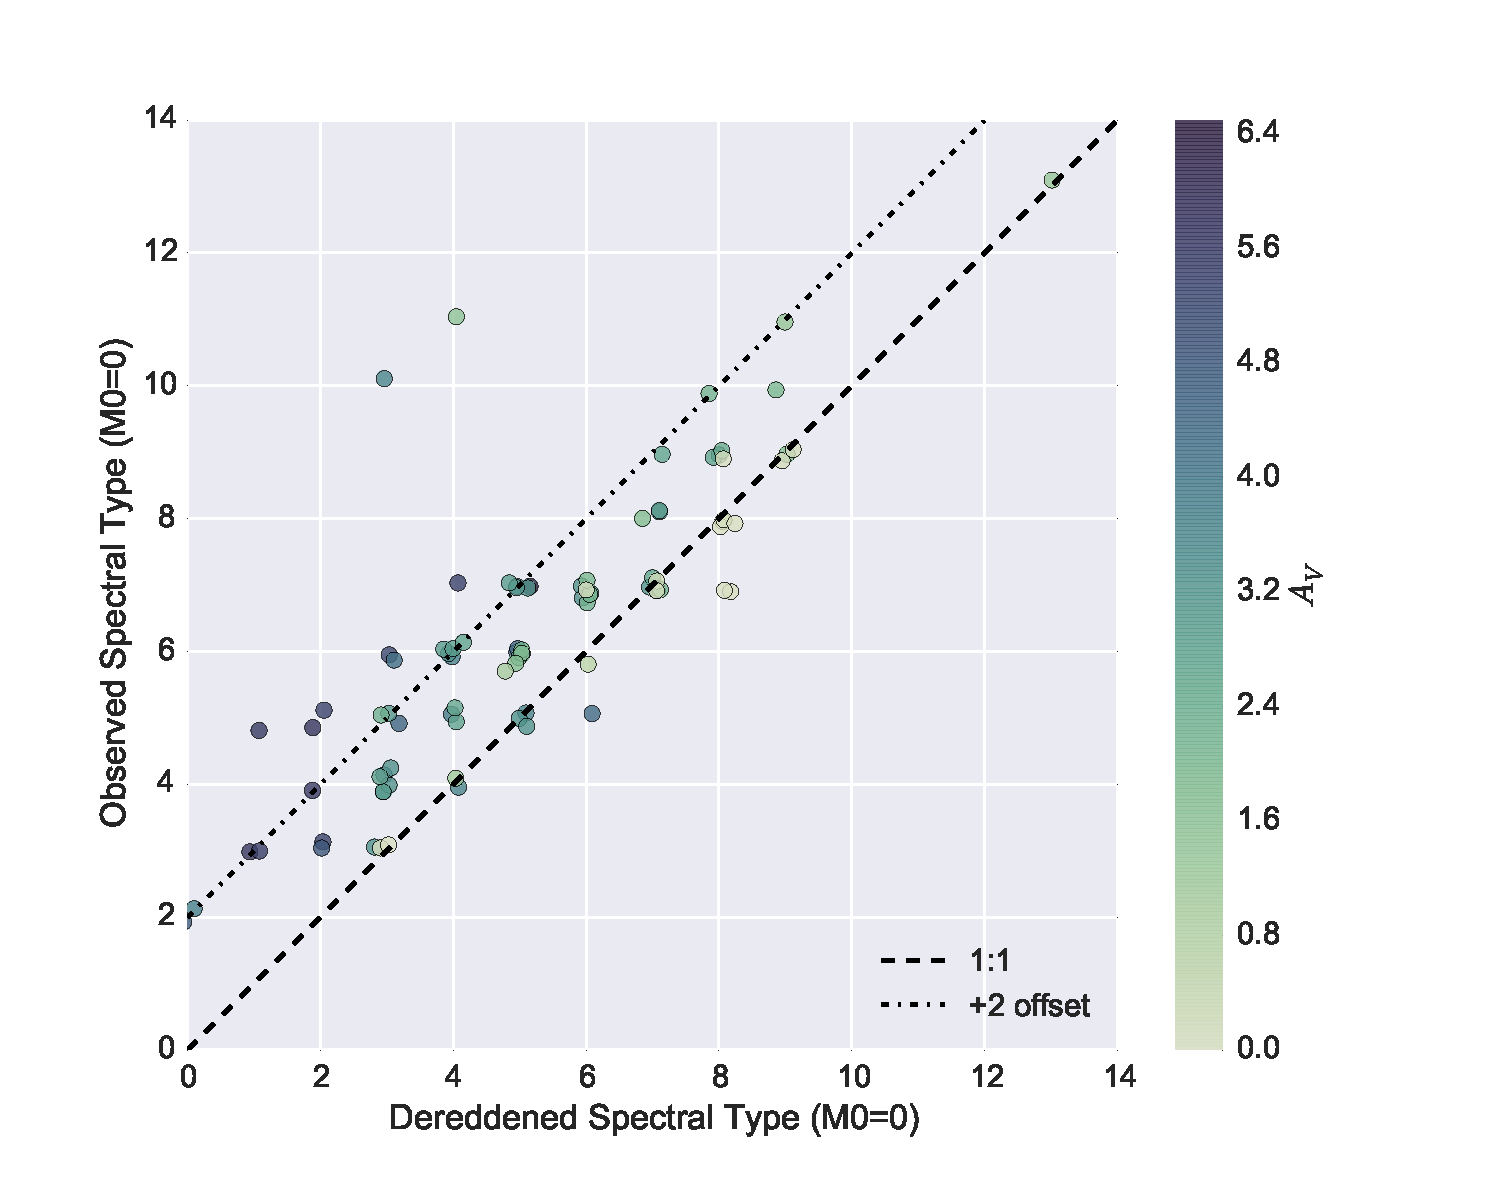
\includegraphics[scale=0.5]{chIMACS/figures/dereddened_spt_comparison}
\end{figure}

For most sources, the second pass spectral type is the final spectral type we assign.  Since the $J-H$ value to which we deredden is fairly constant from M4$-$M9, there is little to gain by re-estimating the extinction from the revised spectral type.  We identify no sources with spectral type later than M9.  

We revised the spectral type for sources that show evidence of youth through their position on the HR diagram (Section \ref{sec_HRD}) or possession of mid-IR excess (Section \ref{sec_SED}).  We compare the YSO candidates to young sources of the same spectral type.  This process is described in Section \ref{sec_individual_sources}.


\begin{figure}[ht!]
\caption{IMACS spectra of new 10 members of \emph{Ophiuchus}.  The members all demsontrate spectroscopic evidence of youth evinced by their weak Na~I feature at 8200$\angstrom$.  Source 2mx\_10919 is missing the Na~I feature but demonstrates exceptionally large H$\alpha$ attributable to accretion.  The spectra have been Gaussian smoothed with a 7$\angstrom$ kernel bandwidth.  All spectra were corrected for telluric absorption.  The spectra are normalized at 7500 $\angstrom$ and offset by 1 in the vertical direction. \label{fig_IMACS_spectra1} }
\centering
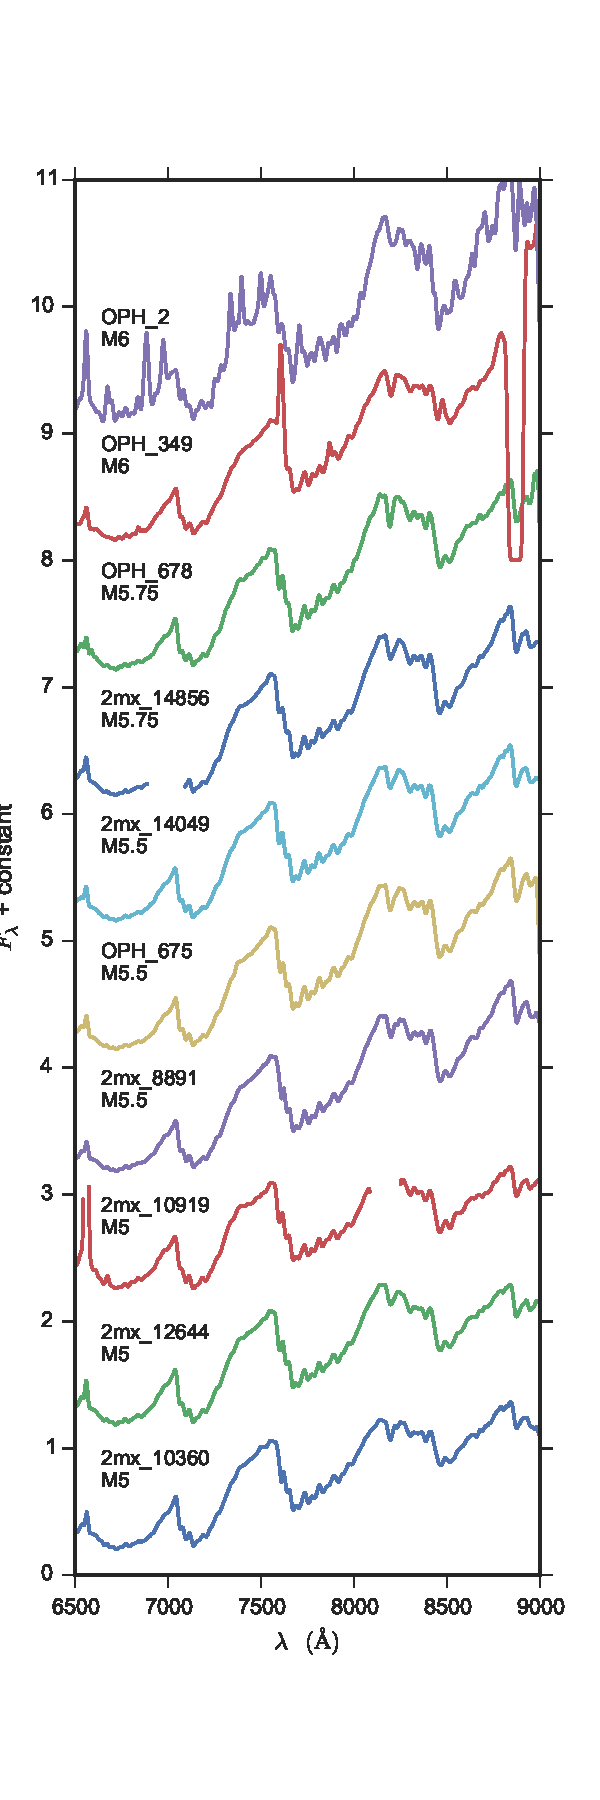
\includegraphics[scale=0.65]{chIMACS/figures/IMACS_spectra_M0_M6}
\end{figure}


\begin{figure}[ht!]
\caption{IMACS spectra of 5 new young brown dwarfs with spectral types M6$-$M8.5.  Same scaling as in Figure \ref{fig_IMACS_spectra1}. \label{fig_IMACS_spectra2} }
\centering
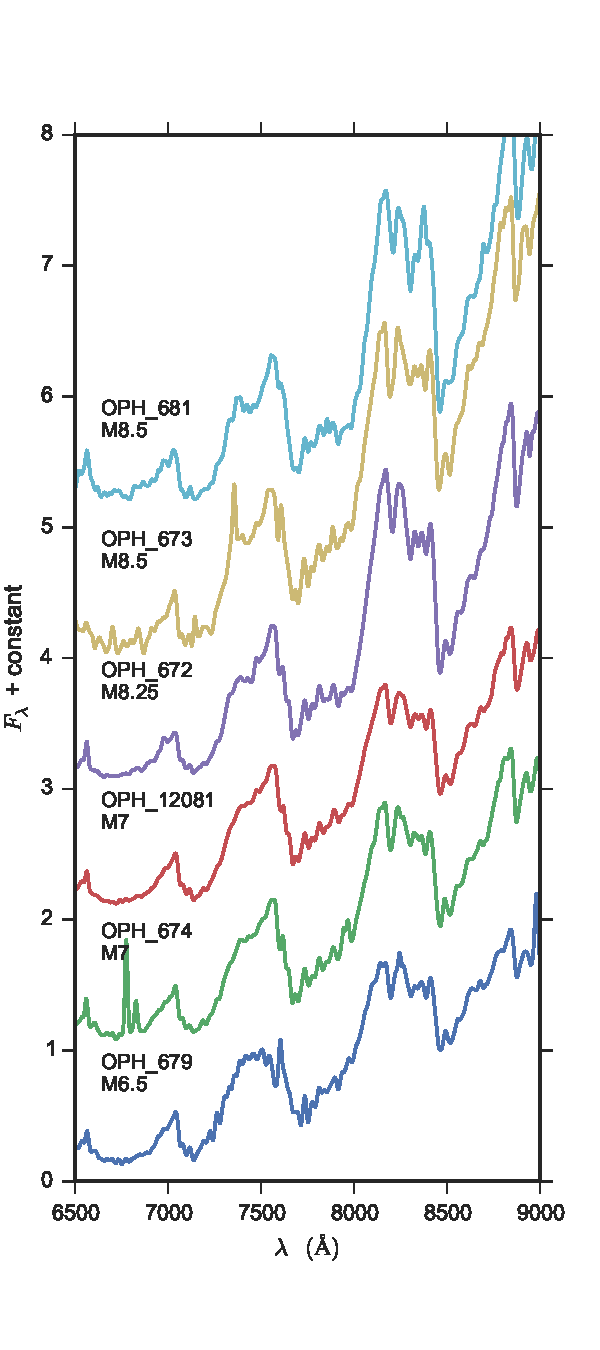
\includegraphics[scale=0.65]{chIMACS/figures/IMACS_spectra_M6_M8p5}
\end{figure}

\subsection{Spectral comparison sample}
We assembled a spectral comparison sample to quantify the gavity-sensitivity of spectral diagnostics as a function of spectral type.  The spectra of dwarfs, giants, and young stars show differences because of their different surface gravities \citep{2012AJ....143..114S}.  A sufficiently large comparison sample will allow the quantification of the spread in spectral indices as a function of spectral type (proxy for temperature) and surface gravity (proxy for age).  The scatter in the spectral indices is important to assign uncertainties in our final age and membership classifications.

We constructed the spectral comparison sample from the RIZzo database \citep{cruz_kelle_2014_10721}, which includes 803 sources- 135 giants, 29 intermediate gravity sources (classified as $\beta$, $\delta$, or $\gamma$ \citep{2009AJ....137.3345C}), and 639 other sources which are mostly old field brown dwarfs or very low mass stars, but contains a few other interlopers and peculiar spectra.  Since the vast majority are field brown dwarfs simply treat them as such.  We crossmatched the RIZzo sample with Simbad to verify their spectral classifications.  A minuscule fraction of the sources had spectral types discordant by more than 1 subtype.  We made no attempt to remove these sources, since we are only using the aggregate properties of the comparison sample.

\subsection{Gravity sensitive indices}
The gravity sensitive Na~I line at 8200 \angstrom$\;$ indicates whether or not our candidate young brown dwarfs are pre-main sequence young substellar objects \citep{1999ApJ...525..466L,2007AJ....134.2398C,2009AJ....137.3345C}.  Figure \ref{fig_NaI_EW} shows the spectral type versus pseudo equivalent width of the Na~I line.  The continuum is ill-defined at low spectral resolution in our heavily line-blanketed spectra in the wavelength region of interest.  Regardless, the index clearly distinguishes between dwarfs and giants taken from the RIZzo comparison sample.

We adopted the continuum and feature indices defined by \citet{2012AJ....143..114S}, namely a central wavelength $\lambda_c= 8190 \angstrom$ and measurement window $\delta \lambda = 22 \angstrom$.  We assigned an uncertainty $\sigma_{EW}$ to the equivalent width by adding in quadrature the uncertainty in the mean of the feature and continuum indices.  We defined a Na~I youth detection as 3$\sigma$ below the bottom 10\% of Na~I equivalent width values of RIZzo dwarfs for a given spectral type.  The 10\% boundary is shown as a solid line in Figure \ref{fig_NaI_EW}.  We also overplot the Na~I EWs of Beta Pic moving group members tabulated in \citet{2012AJ....143..114S}.  Our Na~I EW threshold cuts out some of sources in the 10-20 Myr Beta Pic moving group \citep{2012AJ....143..114S} at spectral types M3 and earlier.  Therefore our Na~I EW threshold is likely overly restrictive at early spectral types, and overly inclusive at late spectral types.  We also compared the Na~I EWs for our sample to those for members of Upper Scorpius \citep{2006AJ....131.3016S}.  Specifically we converted the ratio computed in their Table 1 to an equivalent width, and found a range of about 0.6$-$4.2 $\angstrom$ for spectral types M5 to M8, comparable to the range we see.  Forty two spectra were on the side of the Na~I EW threshold that makes us think they are young.

\begin{figure}[ht!]
  \caption{Na~I 8190 equivalent width as a function of spectral type from M0 to L5.  The sequence shows a clear bifurcation, splitting into groups of relatively high surface gravity (dwarfs, red points at the top), and low surface gravity (giants, blue points at the bottom).  Objects classified as intermediate gravity ($\beta$, $\gamma$, or $\delta$) are shown as purple circles.  Young 10-20 Myr sources in the Beta Pictoris moving group (BPMG, \citet{2012AJ....143..114S}) are shown as large orange circles.  The dotted black line shows the median of the field dwarfs in Rizzo.  The solid black line excludes 90\% of the field objects, and defines our criterion for Na~I EW indicative of youth.  The green squares are young brown dwarf candidates from this work that meet the youth criterion.  The brown triangles are sources that do not meet the criterion for youth.\label{fig_NaI_EW} }
\centering
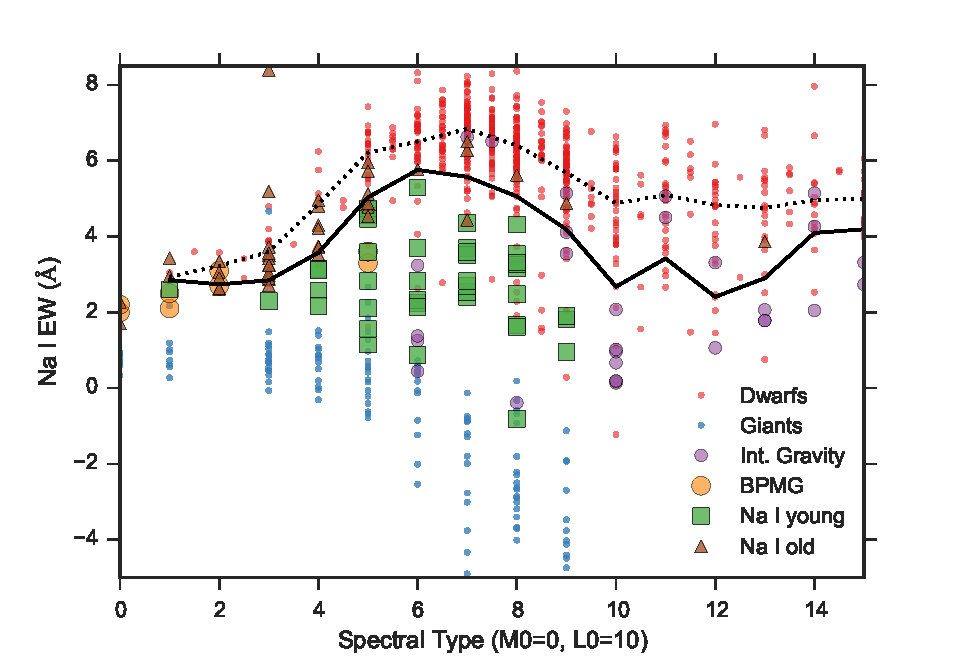
\includegraphics[scale=0.6]{chIMACS/figures/NaI_EW}
\end{figure}

\subsection{H$\alpha$ emission}
We computed the $H\alpha$ equivalent width using the same feature and continuum indices as \citet{2011AJ....141...97W}.  We assigned an uncertainty to the equivalent width in the same way as we did for Na~I- adding the uncertainty in the means of feature and continua values in quadrature.  The choice of an $8 \angstrom$ central wavelength window was comparable to our spectral resolution.  We defined an $H\alpha$ emission detection as exceeding 3$\sigma_{EW}$ over the 90\% of $H\alpha$ EW computed per spectral type bin of the RIZzo sample.  Since emission line EWs are negative, this means more negative than 90\% of the RIZzo sample, for a given spectral type bin, as shown in Figure \ref{fig_Ha_EW}.  Though many sources show $H\alpha$ emission lines, only 15 sources show emission line strengths in substantial excess of the non-accreting comparison sample.

\begin{figure}[ht!]
  \caption{H$\alpha$ equivalent width as a function of spectral type from M0 to L5.  The sequence shows a large spread in values for spectral types later than the M4 transition.  The symbol colors and shapes are the same as in Figure \ref{fig_NaI_EW}.  The dotted black line shows the median of the field dwarfs in Rizzo.  The solid black line excludes 90\% of the field objects, and defines our threshold for H$\alpha$ emission indicative of youth.  The green squares are young brown dwarf candidates from this work that meet this youth criterion at greater than $3\sigma_{EW}$.  The brown triangles are sources that do not meet the criterion. \label{fig_Ha_EW} }
\centering
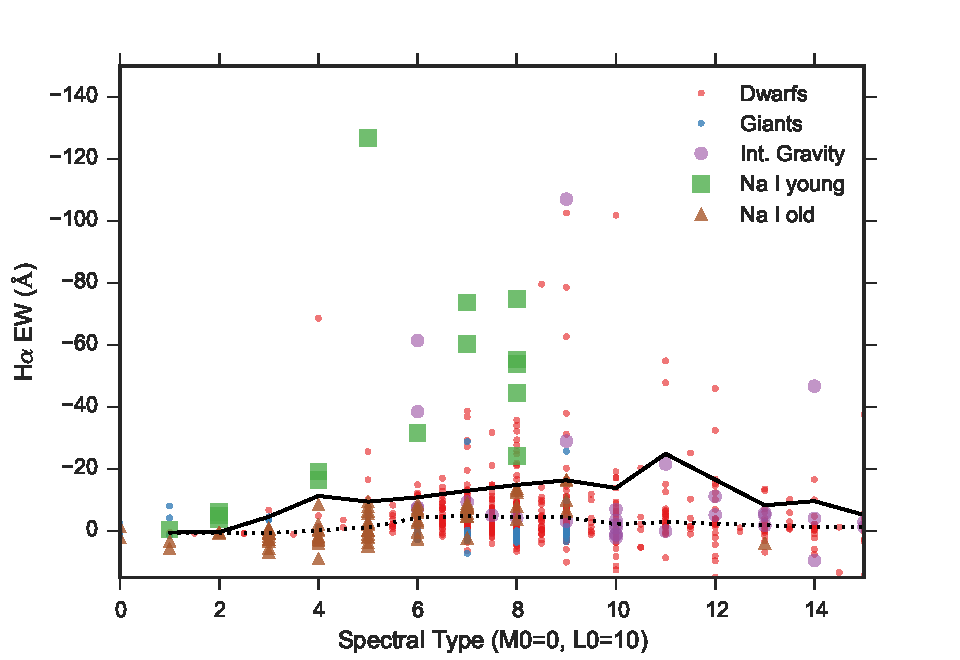
\includegraphics[scale=0.6]{chIMACS/figures/Ha_EW}
\end{figure}


\subsection{Effective Temperatures}
We use the \cite{2003ApJ...593.1093L} effective temperature scale for spectral types M1-M9.  For M0 we assume $T_{\mathrm{eff}}= 3770$ \citep{2013ApJS..208....9P}.  We ignore sources with spectral types earlier than M0.  For sources with non-integer spectral substypes, we linearly interpolate between adjacent integer subtypes.  We assign an uncertainty in temperature of 150 K which includes the uncertainty of the spectral classification.  The systematic uncertainty in the temperature scale is even larger, as noted by \citet{2013ApJS..208....9P} and \citet{2010ApJS..186...63R}.

\subsection{Luminosities}
We computed luminosities for all 71 sources with late M or L spectral types.  We computed absolute magnitudes assuming a distance of 125 pc \citep{2008ApJ...675L..29L}, apparent $J-$ magnitudes corrected for extinction, and $J-$band bolometric corrections.  We set the bolometric correction as a function of spectral type in the following way.  For spectral types M5 or earlier we used $BC_J$ reported by \citep{2013ApJS..208....9P}.  For spectral types M5.5 and later we used the mean $BC_J$ per spectral type bin reported in \citet{2002AJ....124.1170D}.  We linearly interpolated between data points for fractional spectral subtypes not reported in either \citet{2002AJ....124.1170D} or \citet{2013ApJS..208....9P}.


\subsection{Extinction and position in the HR Diagram}
\label{sec_HRD}
Equipped with derived effective temperatures and luminosities, we placed all 71 late type sources on an HR diagram.  Figure \ref{fig_HRD_NaI_Ex} shows the HR diagram with the pre-main sequence (PMS) evolutionary model tracks of \citep{1998A&A...337..403B,2002A&A...382..563B}.  The dotted lines are logarithmically spaced model isochrones from 1 Myr to 1 Gyr.  The solid black lines show the evolutionary track for sources down to 20 $M_{Jup}$.  The key idea from this Figure is that our sample is split into two populations- those below the main sequence and those above the main sequence.  Below the main sequence, sources are likely to be warmer, more distant background dwarfs.  Alternatively, a source can have a position in the HR diagram below the main sequence if it has a nearly edge-on disk.  These sources would have evidence for a mid-IR excess.  Sources OPH\_349 and OPH\_2 demonstrate potential edge-on disks.  Sources above the main sequence could be in the foreground, so membership assignment also requires evidence of low surface gravity from the optical spectroscopy.  Table \ref{tbl_members_phot} lists the properties for the 16 sources that we define as members.

%\begin{landscape}
%	%%%%%%%%%%%%%%%%%%%%%%%%%%%%%%%%%%%%%%%%
% TABLE - Scores
%%%%%%%%%%%%%%%%%%%%%%%%%%%%%%%%%%%%%%%%
\begin{deluxetable}{lrrp{4cm}cccccc}
\tablecolumns{10}
\tabcolsep=0.11cm
\tabletypesize{\footnotesize}
\tablecaption{Photometry from this work\label{tbl_members_phot}}
\tablewidth{0pt}
\tablehead{
\colhead{Name} &
\colhead{RA} &
\colhead{DEC} &
\colhead{Alt. Names} &
\colhead{Ref.} &
\colhead{$Q$} &
\colhead{$I$} &
\colhead{$J$} &
\colhead{$H$} &
\colhead{$K$} } 
\startdata

 2mx\_10919 &  245.45202 & -23.67426 &  2M J16214848$-$2340273, [AKC2006] 9, [EDJ2009] 740 &  (1,2) & -0.91$\pm$0.15 &  17.50$\pm$0.01 &  13.59$\pm$0.03 &  12.34$\pm$0.03 &  11.69$\pm$0.02 \\
 2mx\_12644 &  245.56067 & -23.78650 &  \ldots &  \ldots & -0.27$\pm$0.07 &  16.19$\pm$0.01 &  12.85$\pm$0.03 &  11.89$\pm$0.02 &  11.41$\pm$0.03 \\
 2mx\_14856 &  245.68725 & -23.28707 &  2M J16224494-2317134, [AKC2006] 13, [EDJ2009] 748 &  (1,2,6) &  \ldots &  17.07$\pm$0.01 &  13.68$\pm$0.03 &  12.74$\pm$0.02 &  12.25$\pm$0.03 \\
 2mx\_10360 &  245.41609 & -23.19431 &  \ldots &  \ldots & -0.85$\pm$0.05 &  15.75$\pm$0.01 &  12.50$\pm$0.03 &  11.57$\pm$0.02 &  11.12$\pm$0.02 \\
   OPH\_673 &  245.42743 & -23.60256 &  \ldots &  \ldots & -0.91$\pm$0.07 &  19.68$\pm$0.01 &  15.04$\pm$0.01 &  13.97$\pm$0.01 &  13.25$\pm$0.01 \\
   OPH\_674 &  245.59602 & -24.11968 &  \ldots &  \ldots & -0.67$\pm$0.01 &  18.96$\pm$0.01 &  14.80$\pm$0.01 &  13.83$\pm$0.01 &  13.18$\pm$0.01 \\
   OPH\_678 &  245.31862 & -24.29600 &  \ldots &  \ldots & -0.69$\pm$0.01 &  18.42$\pm$0.01 &  14.81$\pm$0.01 &  13.96$\pm$0.01 &          \ldots \\
   OPH\_675 &  245.31889 & -23.60123 &  \ldots &  \ldots & -0.86$\pm$0.07 &  17.35$\pm$0.01 &  13.77$\pm$0.01 &  12.94$\pm$0.01 &          \ldots \\
  2mx\_8891 &  245.32603 & -23.18708 &  \ldots &  \ldots & -1.09$\pm$0.05 &  15.33$\pm$0.01 &  12.25$\pm$0.03 &  11.43$\pm$0.02 &  10.96$\pm$0.02 \\
 2mx\_14049 &  245.64313 & -23.38955 &  \ldots &  \ldots &         \ldots &  16.02$\pm$0.01 &  12.45$\pm$0.02 &  11.64$\pm$0.02 &  11.23$\pm$0.02 \\
   OPH\_679 &  245.25929 & -23.97774 &  2M J16210222$-$2358395 & (3) & -0.73$\pm$0.01 &  18.27$\pm$0.01 &  14.63$\pm$0.01 &  13.79$\pm$0.01 &  13.25$\pm$0.01 \\
   OPH\_681 &  245.81346 & -23.78497 &  \ldots &  \ldots & -1.09$\pm$0.06 &          \ldots &  15.10$\pm$0.01 &  14.21$\pm$0.01 &  13.56$\pm$0.01 \\
   OPH\_349 &  245.49823 & -23.26736 &  [JJK2008] J162159.55$-$231602.5 &  (4) & -0.58$\pm$0.02 &  19.25$\pm$0.01 &  16.32$\pm$0.01 &  15.67$\pm$0.01 &  15.36$\pm$0.01 \\
 OPH\_12081 &  245.39963 & -23.91767 &  2M J16213591$-$2355035, [SCH2006] J16213591-23550341 &  (5) & -1.06$\pm$0.01 &  17.10$\pm$0.01 &  13.79$\pm$0.01 &  13.16$\pm$0.01 &  12.72$\pm$0.01 \\
     OPH\_2 &  245.56548 & -23.50553 &  \ldots &  \ldots & -1.01$\pm$0.12 &  20.66$\pm$0.07 &  17.63$\pm$0.02 &  17.09$\pm$0.02 &  16.90$\pm$0.04 \\
   OPH\_672 &  245.56064 & -23.95042 &  \ldots &  \ldots & -1.03$\pm$0.03 &  18.48$\pm$0.01 &  14.62$\pm$0.01 &  13.91$\pm$0.01 &  13.36$\pm$0.01 \\
\enddata

\tablecomments{$Q$ is the degree of water absorption in the $W-$filter band. The source names containing ``2mx'' are from the 2MASS $JH$ catalog.  The sources with ``OPH'' are from the ISPI $JH$ catalog.}
\tablerefs{
(1)~\citet{allers06}
(2)~\citet{2009ApJS..181..321E}
(3)~\citet{2012ApJ...758...31L}
(4)~\citet{2008ApJ...683..822J}
(5)~\citet{2006AJ....131.3016S}
(6)~\citet{2012ApJ...755...67H}
}

\end{deluxetable}
%\end{landscape}

\begin{figure}[ht!]
  \caption{Pre main sequence HR diagram indicating membership of new young very low mass stars and brown dwarfs to \emph{Ophiuchus}.  The green circles are members based in part on their position in this diagram.  The red squares are sources without evidence for membership, or evidence of non-membership.  Sources OPH\_349 and OPH\_2 are edge-on disks, based on the presence of mid-IR excess, suppressed near-IR and optical colors, and their apparent position below the main sequence in this diagram. \label{fig_HRD_NaI_Ex} }
\centering
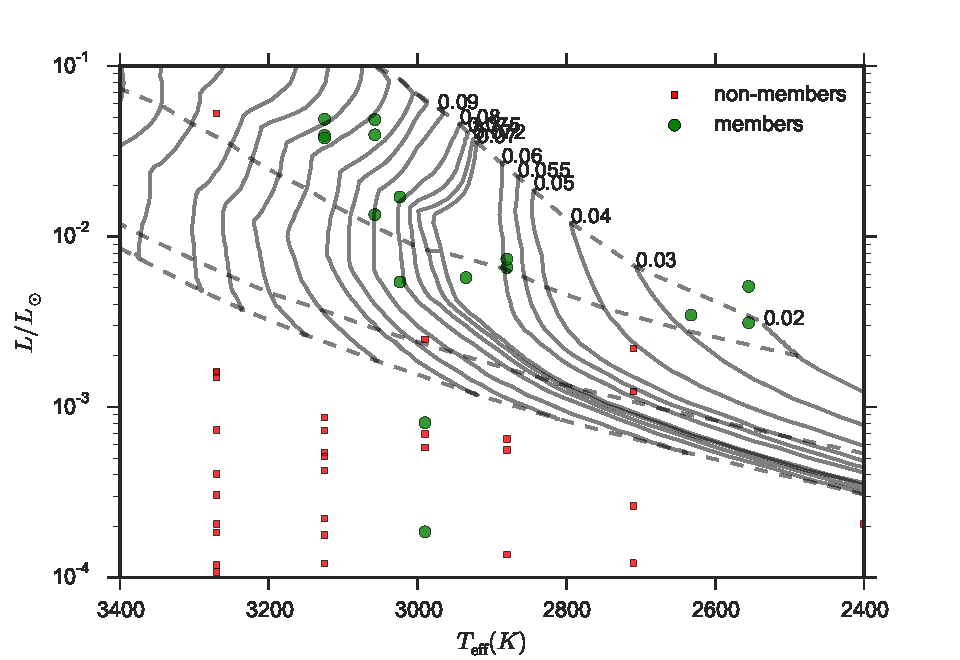
\includegraphics[scale=0.6]{chIMACS/figures/HRD_zoom.pdf}
\end{figure}

\subsection{Spectral Energy Distributions}
\label{sec_SED}

We explored the diversity of mid-IR excess emission properties by constructing spectral energy distributions (SEDs).  Figures \ref{fig_SEDs_9panel} and \ref{fig_SEDs_7panel} show the SEDs for the 16 members in our sample.  Many of the sources do not appear to have mid-IR excess, despite meeting the mid-IR selection criterion for selection.  One main reason is that the sources were detected at 24 $\mu$m.  When designing the survey we targeted the lowest luminosity young brown dwarfs, which should now have detectable photospheres at the distance of Ophiuchus.  The sources we detected are warmer and more luminous than our targets, so we can detect photosphere in some of these sources.


\begin{figure}[ht!]
  \caption{ Spectral energy distributions (SEDs) of 9 members with spectral types M5$-$M6.  The gray circles show the observed photometry.  The green squares show the photometry corrected for the extinction value derived from the first pass spectral typing.  Both the observed and extinction corrected photometric data have been normalized by the extinction corrected $H-$band measurement.  The red dotted line shows the black body with temperature equal to $T_{\mathrm{eff}}$ for each source.  \label{fig_SEDs_9panel} }
\centering
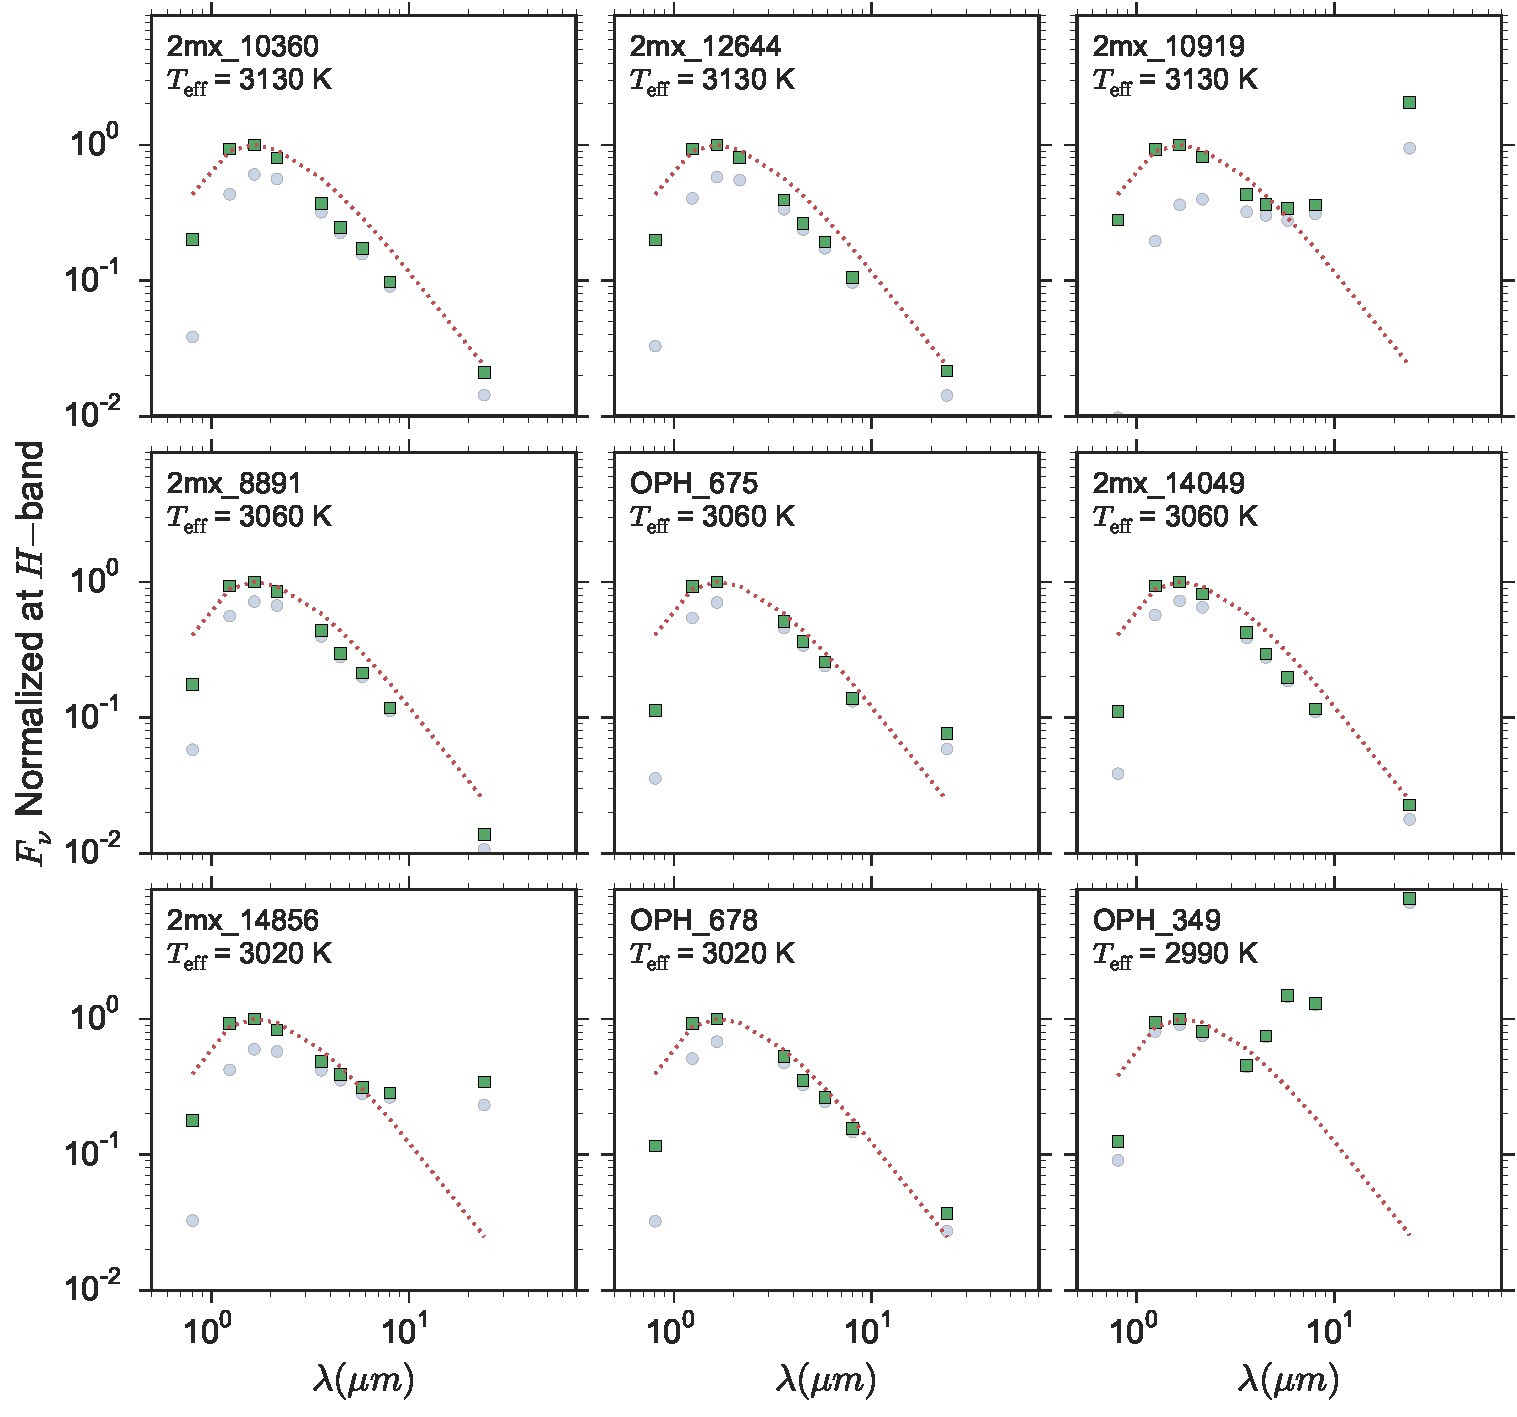
\includegraphics[scale=0.6]{chIMACS/figures/SEDS_9panel}
\end{figure}

\begin{figure}[ht!]
  \caption{ Spectral energy distributions (SEDs) of 7 members with spectral types M6-M8.5.  The plots have the same symbols and scaling as in Figure \ref{fig_SEDs_9panel}.  \label{fig_SEDs_7panel} }
\centering
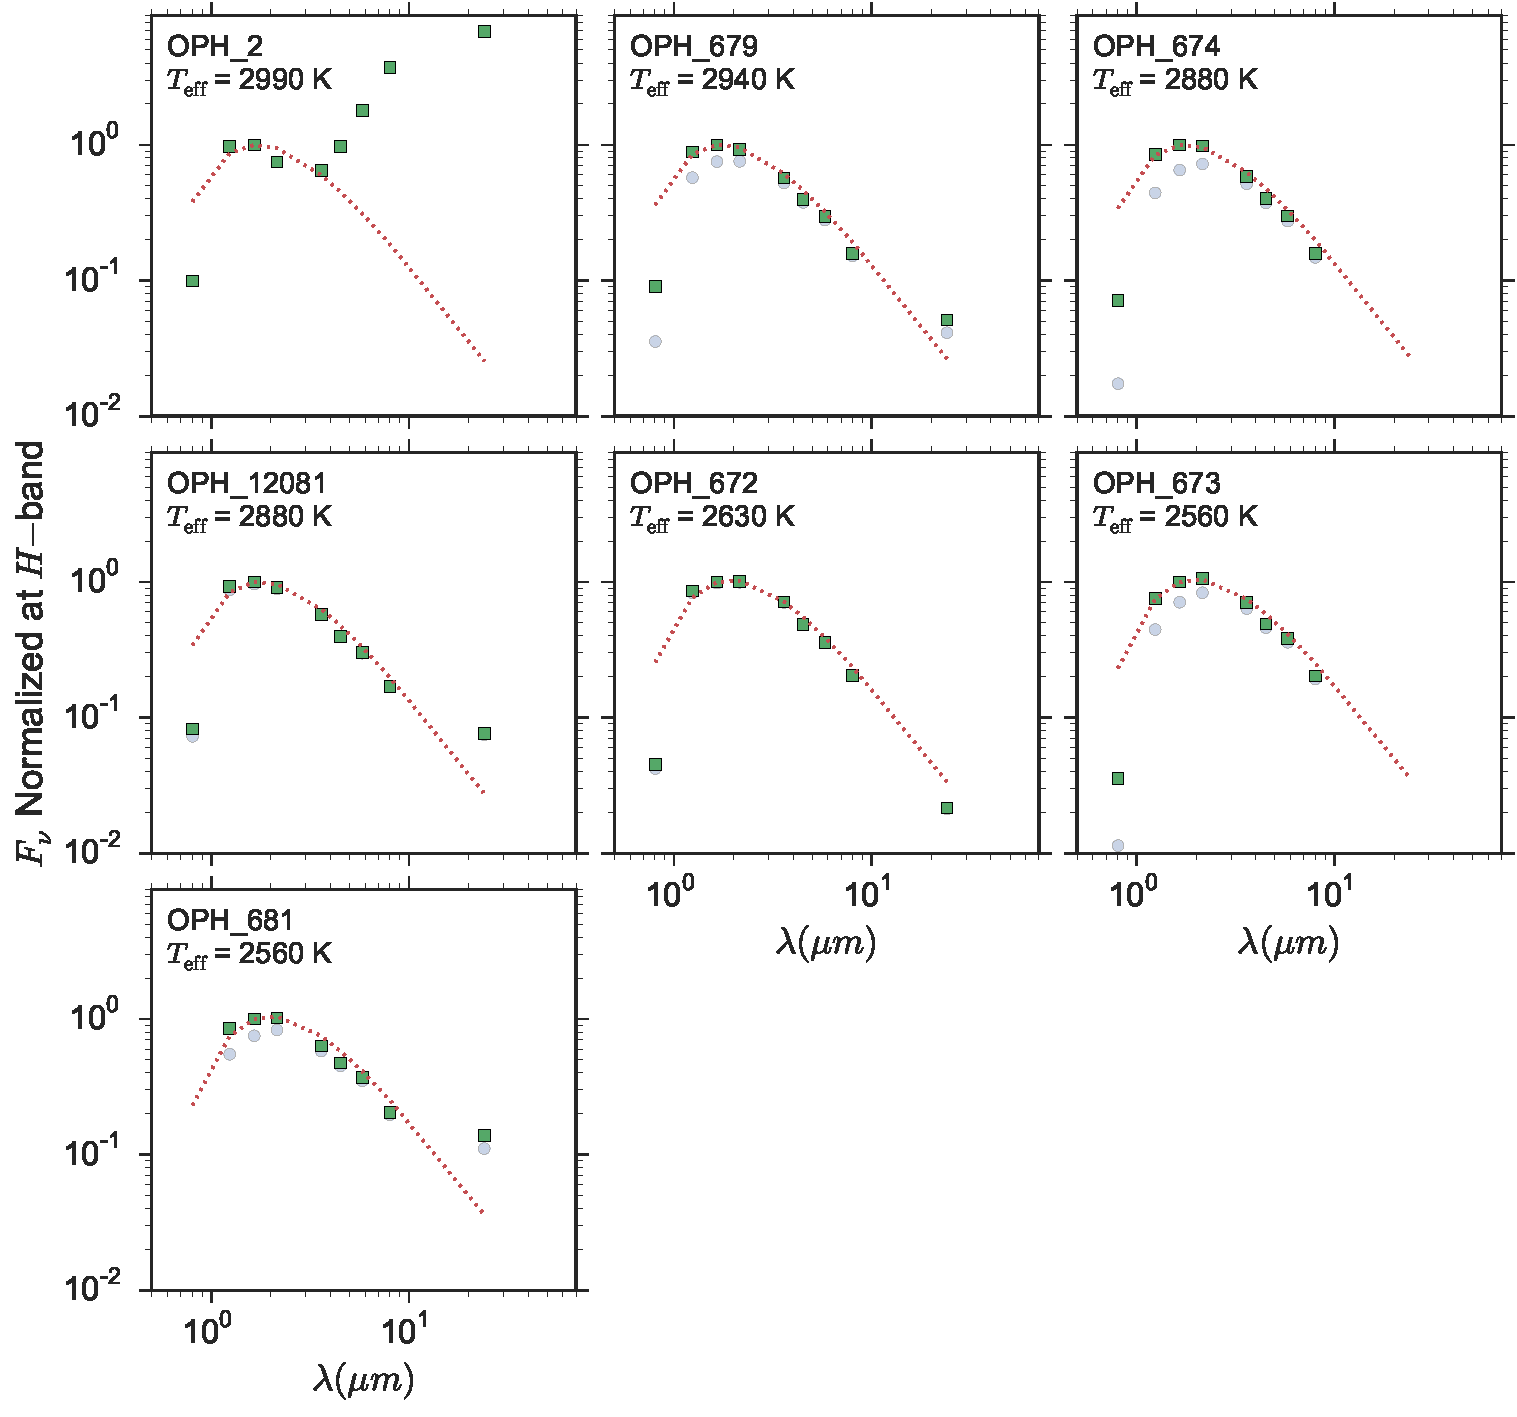
\includegraphics[scale=0.6]{chIMACS/figures/SEDS_7panel}
\end{figure}

%------------------------------------------------------------------------------------------
\section{Results}
%------------------------------------------------------------------------------------------
\subsection{Whittling down from 71 to 10-15}
We adopted a holistic approach to assigning membership to the 71 targets to arrive at 16 sources with confident evidence for membership.  An additional 3 sources are consistent with membership, but lack have spectral types M4 or earlier, which makes their Na~I equivalent widths difficult to distinguish between dwarfs and YSOs.  The remainder of targets have evidence for high gravity features and/or are below the main sequence line and are therefore deemed dwarf contaminants.  Table \ref{tbl_members_phys} lists the derived properties for the final sample of 16 members.  

%\begin{landscape}
%	%%%%%%%%%%%%%%%%%%%%%%%%%%%%%%%%%%%%%%%%
% TABLE - Scores
%%%%%%%%%%%%%%%%%%%%%%%%%%%%%%%%%%%%%%%%
\begin{deluxetable}{lccccccccc}
\tablecolumns{10}
\tabcolsep=0.11cm
\tabletypesize{\footnotesize}
\tablecaption{Spectral classification and derived properties of our sample\label{tbl_members_phys}}
\tablewidth{0pt}
\tablehead{
\colhead{Name} &
\colhead{Priority} &
\colhead{Sp. Type} &
\colhead{$A_V$} &
\colhead{$T_{\mathrm{eff}}$} &
\colhead{$\log L/L_{\odot}$} &
\colhead{H$\alpha$ EW} &
\colhead{Na~I EW} &
\colhead{SED Class} &
\colhead{Night} \\
\colhead{} &
\colhead{} &
\colhead{} &
\colhead{} &
\colhead{K} &
\colhead{} &
\colhead{$\angstrom$} &
\colhead{$\angstrom$} &
\colhead{} &
\colhead{YYYYMMDD} 
}
\startdata
 2mx\_10919 &                   1 &       M5 &  7.1 &  3130 &    -1.4 &     -126.8 &  22.0$\pm$0.3 &        II &    20120513 \\
 2mx\_12644 &                   8 &       M5 &  4.1 &  3130 &    -1.4 &       -7.9 &   2.1$\pm$0.1 &       III &    20120513 \\
 2mx\_14856 &                   3 &    M5.75 &  4.0 &  3020 &    -1.8 &       -8.3 &   2.4$\pm$0.1 &        II &  20120513-4 \\
 2mx\_10360 &                   7 &       M5 &  3.8 &  3130 &    -1.3 &       -6.5 &   2.8$\pm$0.1 &       III &  20120513-4 \\
   OPH\_673 &                   5 &     M8.5 &  4.1 &  2560 &    -2.3 &      -13.9 &   4.3$\pm$0.1 &       III &    20120513 \\
   OPH\_674 &                   5 &       M7 &  4.4 &  2880 &    -2.2 &      -13.2 &   3.5$\pm$0.1 &       III &    20100617 \\
   OPH\_678 &                   5 &    M5.75 &  3.6 &  3020 &    -2.3 &       -4.8 &   3.5$\pm$0.1 &       III &    20120514 \\
   OPH\_675 &                   5 &     M5.5 &  3.4 &  3060 &    -1.9 &       -7.2 &   2.8$\pm$0.1 &       III &    20120514 \\
  2mx\_8891 &                   7 &     M5.5 &  2.9 &  3060 &    -1.3 &       -6.1 &   2.2$\pm$0.1 &       III &  20120513-4 \\
 2mx\_14049 &                   8 &     M5.5 &  2.8 &  3060 &    -1.4 &       -6.7 &   2.3$\pm$0.1 &       III &  20120513-4 \\
   OPH\_679 &                   5 &     M6.5 &  3.2 &  2940 &    -2.2 &       -7.4 &   3.6$\pm$0.2 &       III &    20120513 \\
   OPH\_681 &                   5 &     M8.5 &  2.3 &  2560 &    -2.5 &       -6.5 &   1.0$\pm$0.2 &       III &    20110707 \\
   OPH\_349 &                   4 &       M6 &  1.5 &  2990 &    -3.1 &       -8.6 &   2.1$\pm$0.1 &        EO &    20100617 \\
 OPH\_12081 &                   6 &       M7 &  1.0 &  2880 &    -2.1 &       -7.9 &   2.8$\pm$0.1 &       III &    20110707 \\
     OPH\_2 &                   1 &       M6 &  0.4 &  2990 &    -3.7 &      -44.5 &   1.7$\pm$0.1 &        EO &    20120514 \\
   OPH\_672 &                   5 &    M8.25 &  0.9 &  2630 &    -2.5 &      -16.6 &   1.9$\pm$0.2 &       III &    20110707 \\
\enddata

\tablecomments{Typical uncertainties are about 0.2 in $A_V$, 150 K in $T_{\mathrm{eff}}$, 0.2 dex in luminosity, and 0.1 $\angstrom$ in EW.  The SED Class refers to the mid-IR slope, with ``EO'' indicating edge-on disks.}
%\tablerefs{}

\end{deluxetable}
%\end{landscape}

\subsection{Discussion of individual sources}
\label{sec_individual_sources}
2mx\_9647 is the earliest spectral type source that meets either of our youth criteria.  It is consistent with a spectral type earlier than M1.  We assign it an M0 spectral type, though it could be a late K type.  There is no evidence of accretion, and the source does not have evidence for mid-IR excess.  The source is above the main sequence and demonstrates an $A_V$ of 3.8, so we reject the interpretation that it is a foreground object.  Still, we cannot confidently assign evidence of youth based on the spectrum, so we mark this source as a candidate.  Its telluric-corrected spectrum looks notably different from the comparison spectra which were not telluric-corrected.  

2mx\_10966 has an M4 spectral type with modest H$\alpha$ emission.  The Na~I equivalent width is weak- more similar to Hn17 \citep{2004ApJ...602..816L}, than 2M J05102396-2800539 \citep{2007AJ....133..439C}, which leads us to assign membership to this object.  Its high $A_V$ supports our interpretation that it is a diskless young member of \emph{Ophiuchus}.

The youth of 2mx\_10500 is firm based on mid-IR excess, its weak Na~I equivalent width, and its $A_V\sim2.7$ and position above the HR diagram.  Its moderate H$\alpha$ lends support to its youth and therefore membership.  Its Na~I is weaker than M4V 2MASS J02193311+1416327 \citep{2003AJ....126.2421C}, and comparable to the 2 Myr M4 Hn17 \citep{2004ApJ...602..816L}.

2mx\_12644 shows a spectral shape comparable to the 2 Myr M5 source T50 \citep{2004ApJ...602..816L}, with comparably weak Na~I absorption.  It has modest H$\alpha$, although not substantially more than active M dwarfs \citep{2011AJ....141...97W}.  

2mx\_10919 is unluckily missing the portion of its spectrum surrounding the 8200 $\angstrom$ Na~I line, but its youth and membership are firm based on the presence of mid-IR excess and whopping H$\alpha$emission.  It has a spectral type of M5, based on its similarities with T50.  2mx\_10919 also has the largest estimated extinction of any source, supporting our interpretation that it is a member of \emph{Ophiuchus}.

2mx\_10360 has spectral features very similar to T50, so we assign an M5 spectral type, and membership to \emph{Ophiuchus} based on its weak Na~I absorption.

2mx\_8891 has a spectrum most similar to chxr84, an M5.5 member of Chamaeleon I \citep{2004ApJ...602..816L}, with comparable Na~I.  Its Na~I is much weaker than the M5.5 dwarf 2MASS J11245327+1322533 \citep{2003AJ....126.2421C}.

OPH\_675 has an M5.5 spectral type based on comparison to the same comparison sources as 2mx\_8891.  OPH\_675 has a slightly deeper appearance of the Na~I line than chxr84 does, but still much less than 2MASS J11245327+1322533, so we assign it youth and therefore membership.  Uncorrected telluric absorption in the comparison spectra could contribute to the slightly deeper appearance of Na~I in our spectra versus those of Luhman and RIZzo.  

2mx\_14049 looks almost identical to OPH\_675.

OPH\_678 looks most similar to ChaH$\alpha$6 \citep{2004ApJ...602..816L}, an M5.75.  OPH\_678 has slightly deeper Na~I than ChaH$\alpha$6 does, but much shallower than field M5.5 2MASS J11245327+1322533.  

2mx\_14856 has mid-IR excess indicative of a disk.  Further, its weak Na~I and moderate H$\alpha$ support its youth.  Its spectral type is most similar to ChaH$\alpha$6, so we assign it spectral type M5.75.

OPH\_679 has a low signal-to-noise ratio spectrum.  Its spectrum is comparable to the Cha I M6.5, iso138 \citep{2004ApJ...602..816L}, with much less Na~I absorption than 2MASS J14450627+4409393 \citep{2003AJ....126.2421C}.  

OPH\_673 also has a low signal-to-noise ratio spectrum.  Its spectral shape and Na~I absorption are comparable to the M8.5 KPNO06 \citep{1998AJ....115.2074B,2003ApJ...593.1093L}.  At this late spectral type, the dwarf comparison spectra exhibit Na~I comparable to their young counterparts, so assigning youth is more challenging.  Still, the Na~I line strength in OPH\_673 and KPNO06 is noticeably shallower than M8.5 dwarf 2MASS J16141557+8211327 \citep{2007AJ....133..439C}.  We tentatively assign it as a member.

OPH\_674 resembles Cha I M7 11123099-7653342 \citep{2004ApJ...602..816L}.  The Na~I line is suficiently weaker than 2MASS J04365019-1803262 \citep{2007AJ....133..439C}, so we assign OPH\_674 as amember.  

The spectrum of OPH\_681 is most similar to M8.5 KPNO06 \citep{1998AJ....115.2074B,2003ApJ...593.1093L}, and firmly weaker than M8.5 V 2MASS J13235206+3014340 \citep{2007AJ....133..439C}.  

OPH\_1 and OPH\_3 were not above the main sequence for their derived $T_{\mathrm{eff}}$ and $L_{\mathrm{bol}}$, but exhibited apparent mid-IR excess in IRAC band 4.  We examined the IRAC band 4 imaging and found that the IRAC4 detections were consistent with spurious structure from cloud nebulosity.  OPH\_3 exhibits strong Na~I and K~I absorption for its M3 spectral type.  The Na~I absorption cannot be reliably distinguished between OPH\_1 and dwarfs of the same spectral type.  Nevertheless, their underluminosity and refuted evidence for a disk lead us to mark these sources as background objects (given their extinction).

OPH\_2 has dramatically rising mid-IR excess emission.  The low signal-to-noise ratio spectrum of OPH\_2 is most similar to that of Cha I M6 chsm1982 \citep{2004ApJ...602..816L}, and has a clear indication of youth from its weak Na~I line.  The moderate H$\alpha$ supports its youth.  Its apparent position below the main sequence leads us to demarcate OPH\_2 as an edge-on disk, and therefore a member.

By the same logic applied to OPH\_2, OPH\_349 is also an edge-on disk.  Specifically, its prominent mid-IR excess and apparent position below the main sequence are dead giveaways.  The spectrum is consistent with an M6 spectral type classification, with Na~I comparable to that of CHSM1982.  The H$\alpha$ is weak in this source.

\subsection{Edge-on disks}
Figures \ref{fig_SEDs_9panel} and \ref{fig_SEDs_7panel} include the conspicuously rising SEDs of sources OPH\_349 and OPH\_2.  These sources demonstrate mid-IR flux increasing with wavelength from 3.6 to 24 $\mu$m.  The sources fall below the the main sequence in the HR diagram, indicating that these sources are most likely edge-on disks.  The IMACS spectrum of OPH\_2 shows strong H$\alpha$ emission.  OPH\_349 is separated by 4" from OPH26571.  Below is the postage stamp images of the pair in different bands.  \cite{2008ApJ...683..822J} identified OPH\_349 during their search for deeply embedded YSOs.  This source is included in their list of candidate edge-on disks, since it exhibited very red mid-IR colors but no associated SCUBA flux.


\begin{figure}[ht!]
  \caption{Images of OPH\_349 with the nearby OPH\_26571.  Images are from right to left: MOSAIC $I-$band, $[3.6]$, $[8.0]$.}
\begin{minipage}[b]{0.3\linewidth}
\centering
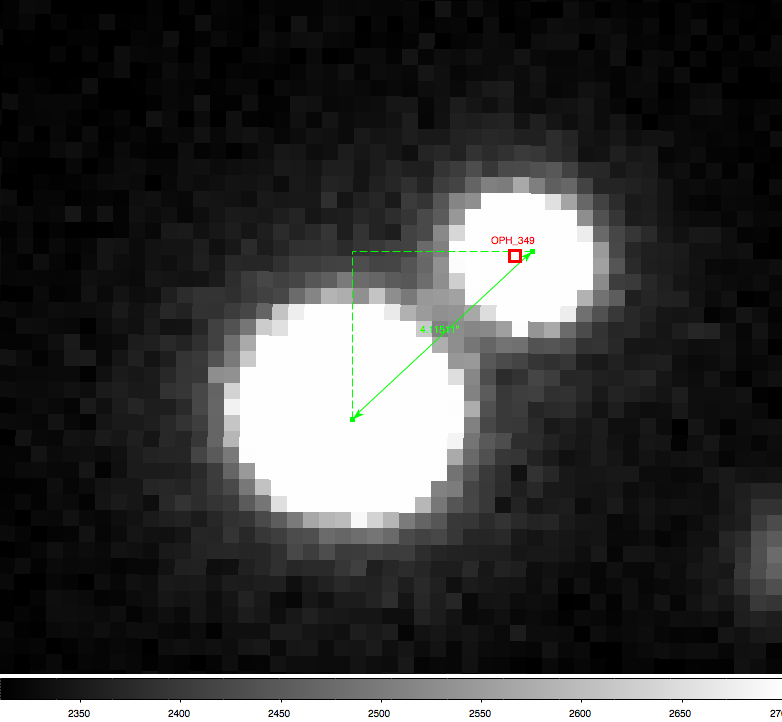
\includegraphics[scale=0.15]{chIMACS/figures/OPH_349_I_image}
\end{minipage}
\hspace{0.5cm}
\begin{minipage}[b]{0.3\linewidth}
\centering
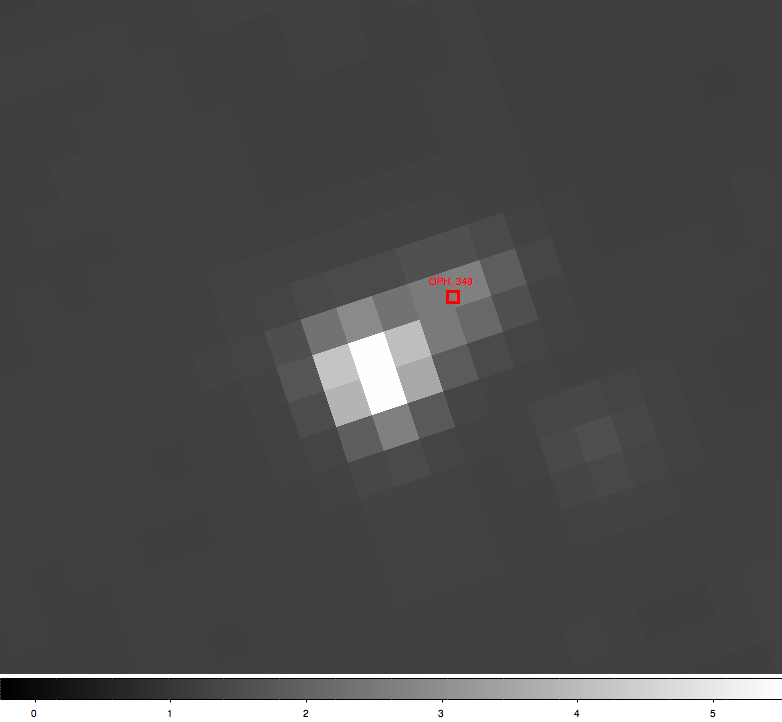
\includegraphics[scale=0.15]{chIMACS/figures/OPH_349_IRAC1_image}
\end{minipage}
\hspace{0.5cm}
\begin{minipage}[b]{0.3\linewidth}
\centering
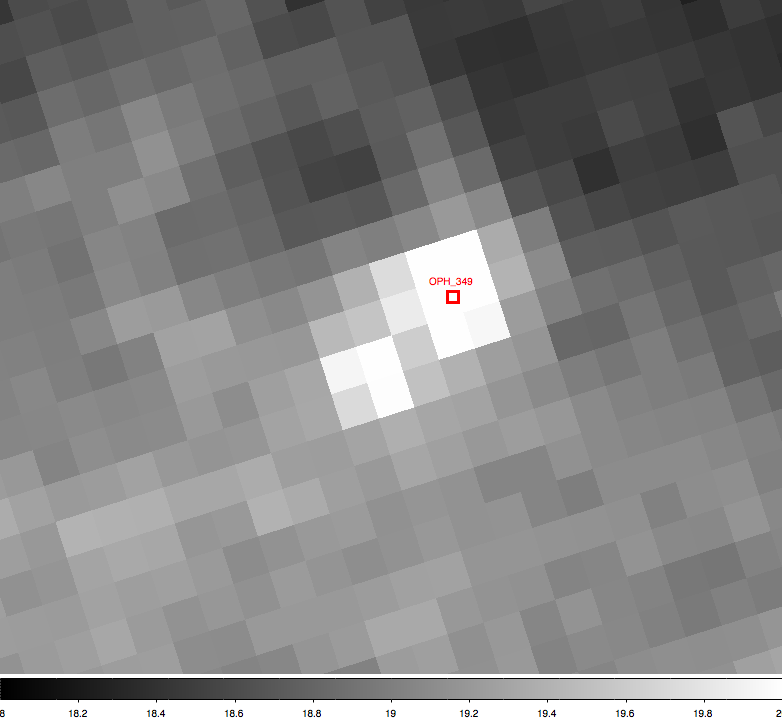
\includegraphics[scale=0.15]{chIMACS/figures/OPH_349_IRAC4_image}
\end{minipage}
\end{figure}

\subsection{Mid-IR colors of diskless new members}

We looked at the distributions of the mid-IR slope of our new members to quantify the diskless and disk-bearing members.  We include in our analysis the mid-IR data of 187 Class I, II, and III Taurus members with spectral types later than M0 \citep{2010ApJS..186..111L}.  The large number of Taurus members allows us to construct a kernel density estimate in a plot of $[3.6]-[8.0]$ versus spectral type, shown in Figure \ref{fig_I1_I4_density}.  The marginal distribution of $[3.6]-[8.0]$ reveals a dichotomy between disk-less Class III sources with $[3.6]-[8.0] \sim 0$ and disk-bearing Class II sources with $[3.6]-[8.0] \sim 1.5$.  The valley in-between the Class II and Class III sources can be understood as a evidence for a short-lived phase of disk-clearing, perhaps through planet formation or photoevaporation.  Despite be sensitive to them, we find no sources in this valley that apparently extends into the sub-stellar regime.  We take this observation as evidence that whatever the mechanism for disk-clearing is, it proceeds similarly in the sub-stellar regime as it does for stellar objects.  

\begin{figure}[ht!]
  \caption{ Distribution of $[3.6]-[8.0]$ as a function of spectral type for new young stellar and substellar objects in this work (white squares with black edges).  The distribution of 187 Class I, II, and III Taurus members with spectral types later than M0 \citep{2010ApJS..186..111L} is shown as the kernel density estimate contours in the background.  The black circles with white edges are the 8 sources towards \emph{Ophiuchus} from \citet{allers06} with spectral types from \citet{2011ASPC..448..633G}.  The white dashed line is constructed from Class III young stellar and substellar objects in $\eta$ Cha, $\epsilon$ Cha, and TWA \citep{2010ApJS..186..111L}, and represents the photospheric colors of young objects.  The two edge-on disks OPH\_2 and OPH\_349 are outliers in this plot.  The two Class II sources are 2mx\_10919 and 2mx\_14856.  The other 12 members are class III sources.  \label{fig_I1_I4_density} }
\centering
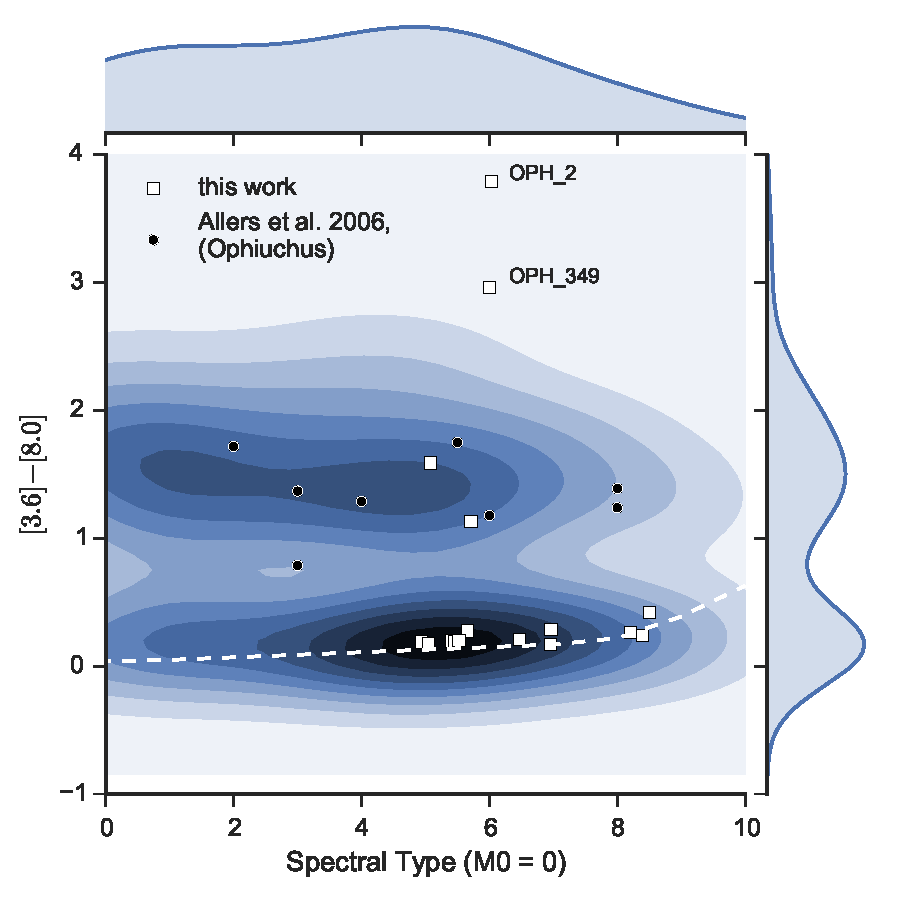
\includegraphics[scale=0.6]{chIMACS/figures/I1_I4_density.pdf}
\end{figure}

We leveraged the class III analogs in our new sample to construct mid-IR photospheric colors of late-type sources.  \citet{2010ApJS..186..111L} construct the photospheric colors of young objects as a function of spectral type with evolved class III objects in $\eta$ Cha, $\epsilon$ Cha, and TWA\footnote{The original table with these values contains an error, see the erratum in \cite{2010ApJS..189..353L}}.  We extend the relationship of \citet{2010ApJS..186..111L} with more late-type sources by combining our sample with theirs.  Figure \ref{fig_midIR_results} shows a close-up on the mid-IR colors of old field dwarfs \citep{2006ApJ...651..502P}, young Taurus members \citep{2010ApJS..186..111L}, and \emph{Ophiuchus} members from \citep{allers06} and this work.  The increasing dichotomy between the background density of Taurus members as a function of wavelength can be understood as the mid-IR excess detaching from the photosphere.  This work has added 3 diskless $\sim$M8 sources, which are among the few diskless objects at such late spectral types for such young ages.  These sources agree with the the \citet{2006ApJ...651..502P} and \citep{2010ApJS..186..111L} to within the measurement uncertainties.


\begin{figure}[ht!]
  \caption{ Mid-IR colors as a function of spectral type for our new members.  New young stellar and substellar objects in this work are white squares with black edges and error bars.  The distribution of 187 Class I, II, and III Taurus members with spectral types later than M0 \citep{2010ApJS..186..111L} is shown as the kernel density estimate contours in the background.  The black circles with white edges are the 8 sources towards \emph{Ophiuchus} from \citet{allers06} with spectral types from \citet{2011ASPC..448..633G}.  The white dashed line is constructed from Class III young stellar and substellar objects in $\eta$ Cha, $\epsilon$ Cha, and TWA \citep{2010ApJS..186..111L}, and represents the photospheric colors of young objects.  The photospheric colors of field dwarfs from \citet{2006ApJ...651..502P} are shown as blue diamonds. 
  The increasing dichotomy between the background density of Taurus members as a function of wavelength can be understood as the mid-IR excess detaching from the photosphere.    \label{fig_midIR_results} }
\centering
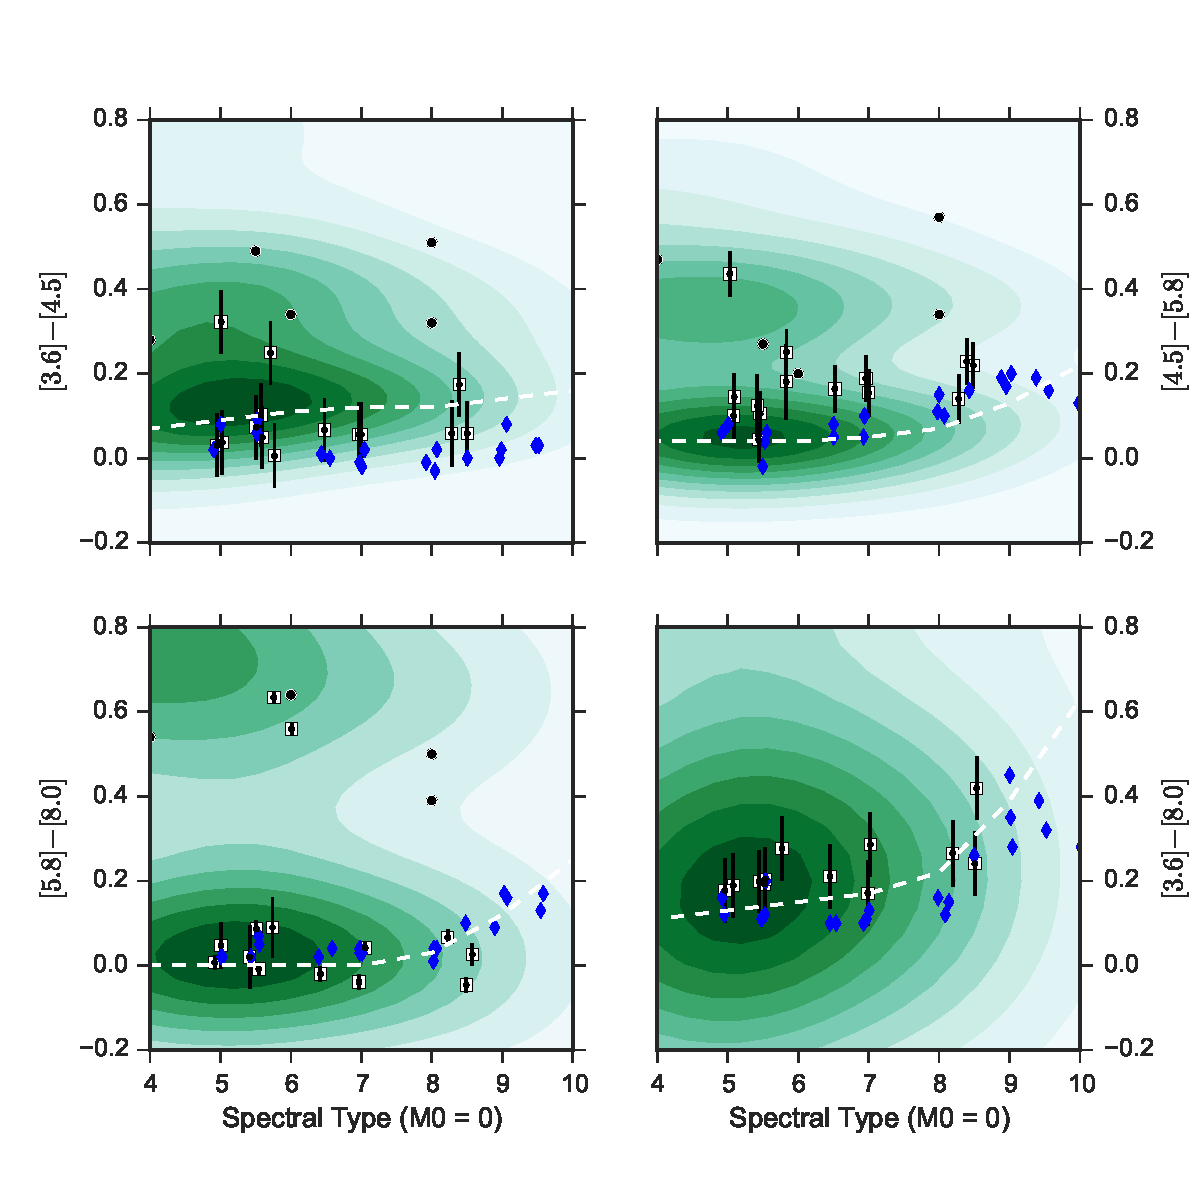
\includegraphics[scale=0.6]{chIMACS/figures/midIR_phot_results.pdf}
\end{figure}

%------------------------------------------------------------------------------------------
\section{Analysis}
%------------------------------------------------------------------------------------------
\subsection{Have we found diskless YBDs?}
One of the main results of this paper is that we have found a large population of diskless young sources.  This discovery shows that 1) disk fractions are probably lower for low-mass stars/brown dwarfs than was previously thought, and 2) brown dwarfs are slightly more common than was previously thought.  Specifically, we detect evidence for disks around 5/14 sources, leading to a disk fraction of 36\%.  Since we slightly favored selection and confirmation towards objects with disks, the true disk fraction could be even lower.  Since most surveys bias selection towards mid-IR excess, diskless brown dwarfs have probably been under-counted, and are therefore slightly more numerous than had been previously thought.


\subsection{How do the properties of the sources scale with luminosity?}
Our final sample consists of 14 young VLMS and BDs.  The lowest luminosity objects are around $2 \times 10^{-3} L_{\odot}$, with the highest luminosity sources at about 10 times that number.  Since our sources span an order of magnitude in luminosity, we can probe to see whether any source properties scale with luminosity.  First, we have found some Class III analogs-- sources that have already depleted their disks.  Those sources with mid-IR excess show relatively weak excess.  This can be understood as a radiative transfer effect \citep{2012A&A...539A...9M,2009MNRAS.394L.141E}.  \cite{allers06} interpreted their disk excess scaling with luminosity as a constant solid angle intercepted by the disk.  We do not see clear evidence for that phenomenon in our sample, but we have few disks.  

\subsection{What would we have selected if we had used selection criteria similar to other authors?}
This is a tough question to answer.  The various surveys for young brown dwarfs use different combinations photometric systems, and different permutations of successive color cuts.  It's relatively hard to reproduce the selection of other surveys with our available data, unless we restrict ourselves to large survey data (like WISE, 2MASS, c2d).  

Although quantitative comparison is not possible, a qualitative view still offers some understanding here.  The main difference between our sample and others' is that we find a large fraction of diskless sources.  Any survey that relies on mid-IR excess as a criterion for selection would therefore have missed the large fraction of our detections.  We use this fact to make the follow main result of this article.  Brown dwarfs are slightly more common than was previously though, since we have uncovered a relatively large fraction of diskless objects, that would have evaded other surveys.  Another relevant question along these lines is: ``What would we have selected (or mistakenly ranked highly) if did not have access to the  $W-$filter?''.


\subsection{What were all the other contaminants and why did they enter our sample?}
Most of the sources in the spectroscopic sample that are not confirmed as members in our work are background sources, based on their apparent position below the main sequence.  This makes sense, since the $W-$ filter does not select based on youth, but only late spectral type.

\subsection{Performance of the $W-$ filter}

The $Q$ value is designed to correlate roughly with the spectral type.  We use our derived spectral types to evaluate to what extent the $W-$ filter $Q$ value correlated with spectral type.  Figure \ref{fig_W_results} shows $Q$ as a function of spectral type for both our confirmed young members (green squares) and late-type non-members.  We fit a straight line to the members, which have higher precision on their spectral type classification than the non-members.  The fit shows a trend in the right direction: later type sources have larger $Q$ values on average.  We do not use the uncertainty in the $Q$ value in the straight-line fits.  The trend is even stronger in the same direction, if the measurement uncertainty is included in the fit.  Still, the large number of non-members that disobey the fit point to the role of measurement uncertainty both in $Q$ and in the coarse spectral typing of non-members with \emph{The Hammer}.  We find no late-type sources with $Q>0$ (excluding a known wide binary brown dwarf 1622-2405, which has been omitted from the figure, since its $W-$band photometry is likely affected by its companion.)  Most of the non-members and all but 1 of the members have $Q<-0.5$, which defined the lower boundary of our $W-$band selection method.  

\begin{figure}[ht!]
  \caption{ Performance of the $W-$filter $Q$ value as a function of spectral classification.  The blue squares are members, the green squares are late-type non-members.  The left portion of the plot shows the probability density function for the parent catalog of 31348 sources with a $W-$filter measurement (red stepped histogram with fine binning centered at $Q=0.0$).  The probability density distribution of all the late-type non-members is shown as the blue stepped histogram with coarse binning. We have excluded the outlier 1622-2405, a known binary brown dwarf, from the figure.  The spectral type positions have a small ($\sim0.1$ spectral subtype jitter added to them to displace the points for legibility).\label{fig_W_results} }
\centering
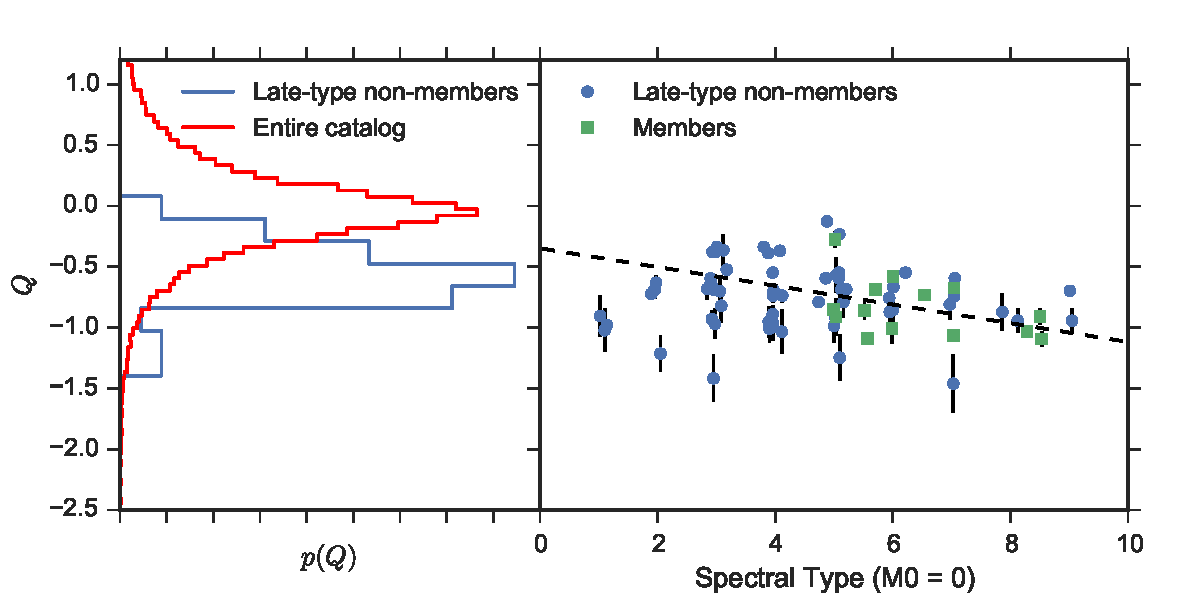
\includegraphics[scale=0.6]{chIMACS/figures/W_filter_results}
\end{figure}

\subsection{Prospects for future surveys}
Given all the challenges and biases associated with photometric selection, it is instructive to ask ``What is the prospect for improving selection strategies in future surveys?''  The best possible strategy would be to have high precision proper motions and parallaxes to kinematically peg sources to the cloud of interest.  Parallaxes would be even better for deriving accurate luminosities, which would constrain ages and masses even better than we can now.  Unfortunately these low luminosity, red sources are below the detection threshold for \emph{GAIA}.  Proper motions with \emph{Spitzer} are just becoming available, given the long baseline (almost 10 years) from the c2d mission to the present day.  One main challenge of proper motions is the extent to which the cloud motion is distinct from the spread of background objects.  This is an active area of research.

\subsection{What is the range of model-derived masses of all of the sources?}
We plot the sources on an HR diagram, as described previously.  Based on the position of the sources in this diagram we can infer a mass and age.  From inspection of the HR diagram we see that the objects range in inferred ages from 1$-$100 Myr, and inferred masses from 20-450 Jupiter masses.  It appears that source 2mx\_10966 is a bit of an outlier in this chart, which is consistent with its borderline membership since M4's are hard to distinguish based on their Na~I EW alone.  So in fact, this source is most likely misclassified, so let's reject it.  In that case the largest inferred mass in our sample is 0.2 $M_{\odot}$, with no source exhibiting an age older than $\sim80$ Myr.


There are many perils associated with deriving ages and masses in this way.  This strategy assumes the models are accurate, and that secondary effects like accretion history have not occured.  We also assume that chromospheric activity is negligible \citep{2014ApJ...796..119S}.  The uncertainties in spectral classification correspond to errors of $\sim100$ K, which can change masses by factors of 50\% or more.  The luminosities depend on the assumed distance, extinction, spectral-type dependent bolometric corrections, and the observed $J-$ band photometry.  The largest uncertainty from those four are the distance and extinction.  We dereddened to the $J-H$ values assumed for the first pass spectral type.  There is a large intrinsic spread in $J-H$.  So based on this large uncertainty, the luminosities could change by 50\% or more, changing the ages by factors of 3 or more.  


\subsection{What can we say, if anything, about the IMF?}

Our survey was \emph{exceptionally} sensitive to very low luminosity substellar objects and yet we did not find them.  We use this very powerful sensitivity and non detection to conclude that these objects are simply not there.  That is to say, the star formation process is inefficient at producing objects less than 20 Jupiter mass objects.  

The one caveat to this claim is that since our survey was in the optical, the depth is limited by extinction and not the intrinsic source density.  This is true, however we emphasize that due to the variability of extinction \citep{2008A&A...489..143L}, and the low average extinction towards our survey region, we would expect at least \emph{some} detections if these very low luminosity sources existed in the wild.  But we find zero, affirming our claim that these sources are exceptionally rare.  

A \emph{true} understanding of the stellar and substellar initial mass function (IMF) requires careful consideration of biases and selection effects, so we make no attempt to derive a shape of the IMF from our sample.  For example, survey selection methods that bias against detection of luminous or underluminous sources will directly flow down to an inaccurate derivation of the IMF.  Since our selection methods involved many different factors, it is a bit tricky to disentangle how these effects might have biased the selections towards and away from the IMF.  In the same vein, the heterogeneity of selection might average down the biases, so that, \emph{on average}, we have selected a representative sample of sources.

With all those provisos, we will speculate here about the IMF.  Assuming all the sources were coeval, and they are members of \emph{Ophiuchus}, the latest spectral type object corresponds to the lowest mass object.  OPH\_673 is an M8.5, giving it an effective temperature around 2500 K \citep{2003ApJ...593.1093L}, and a mass around 20-30 $M_{Jup}$-- firmly substellar.  Objects this low mass have been found, but are relatively rare.  We do not find \emph{any} sources with spectral types later than M8.5, despite our ability to detect them.  To demonstrate that ability, Figure \ref{fig_luminosity_dist} shows the distributions of derived luminosities for all 71 of the sources demonstrating M or L spectral types, overplotted with the distributions of the confirmed young objects.

\begin{figure}[ht!]
  \caption{ Distributions of luminosities of all 71 sources demonstrating M or L spectral types, overplotted with the 16 confirmed young stellar objects. \label{fig_luminosity_dist} }
\centering
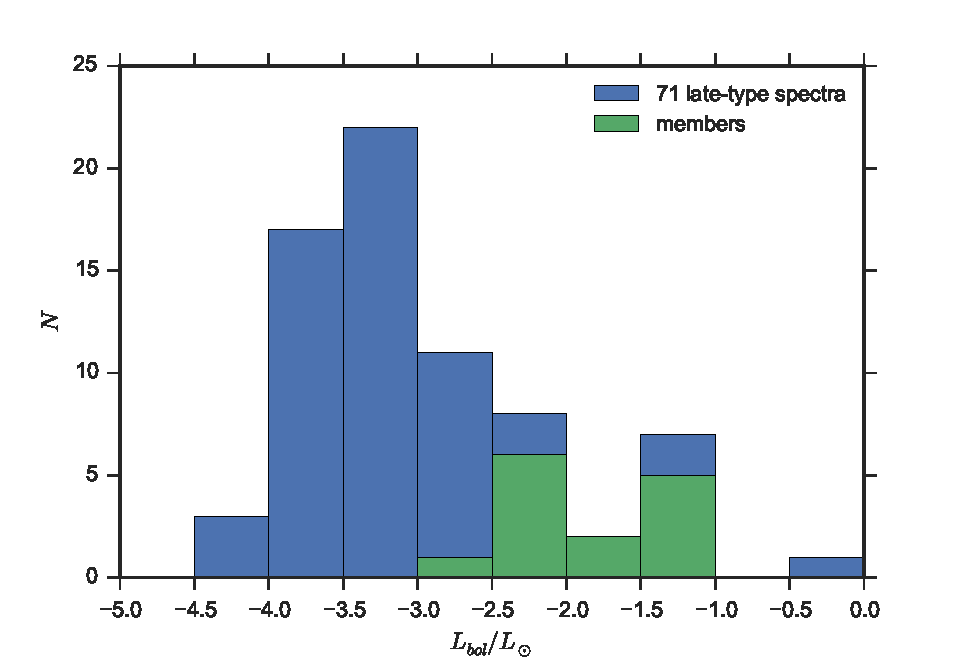
\includegraphics[scale=0.6]{chIMACS/figures/luminosity_histogram}
\end{figure}


\subsection{Is there a higher incidence of edge-on disks in BDs?}
One main result of this work is the identification of two  edge-on disks, our of only 5 disk-bearing sources in our sample.  Taken at face value, 40\% of the disk-bearing sources in our sample have disks.  This result is not a selection effect, since we were sensitive to the substellar photospheres, as demonstrated in our detection of diskless young brown dwarfs.  A 40\% edge-on disk fraction is much higher than the incidence observed in surveys of higher mass stars, in which only a few edge-on disks are found compared to face-on disks.  We interpret this high fraction has tentative evidence that brown dwarf disks have a larger scale height for a given radial position.  This interpretation is consistent with our intuition that the vertical component of gravity should be much lower for a given radial position, and that the disk orientation should be isotropic on the sky.  Of course, the achieved scale height also depends on the degree of turbulence in the disk, so a detailed analysis would have to consider the average temperature and diffusion timescales at a given location in the disk \citep{2012A&A...539A...9M,2009MNRAS.394L.141E}.  However, \emph{on average}, the systematic bias should tend towards higher gravitational scale height for brown dwarf disks, at a given radial distance.

\subsection{Are any of these sources from Upper Sco?}

One of the main potential uncertainties throughout all of this work is the question of whether the young sources belong to the younger \emph{Ophiuchus} or the older \emph{Upper Scorpius}.  Our region sits between these two on the sky, so it's conceivable that some of our detections include a mix of these two populations.  By plotting the projected positions of known objects, we can get an estimate of the surface number density of low mass objects.  Extrapolating roughly from \citet{2006AJ....131.3016S,2012ApJ...758...31L} we estimate that about 2$-$4 Upper Sco objects could be in our region.  This number is consistent with the appears of our HR diagram, in which 4 objects sit substantially lower than the 10 Myr isochrone, but above the 100 Myr isochrone.  The slightly older and more distant population of Upper Sco would be expected to occupy a region in this vicinity.  The fact that the disks are more evolved is consistent with an interpretation of an older, $\sim5$ Myr population.

\subsection{How do these sources compare to Allers et al. 2006?}
All of the candidates in \citet{allers06} exhibited mid-IR excess.  The members reported here are predominantly disk-\emph{less}, based on their photospheric mid-IR colors.  The difference between these two results is wholly due to the disparate selection methods.  Specifically the $W-$ filter offers us the ability to isolate sources with late-type spectra, regardless of their mid-IR photospheric properties.  


%------------------------------------------------------------------------------------------
\section{Conclusions}
%------------------------------------------------------------------------------------------

We have reported on a broad-band survey aimed at the discovery of young brown dwarfs and very low mass stars towards the \emph{Ophiuchus} star forming region.  We present the selection, spectral analysis, discovery, spectral types, luminosities, and physical characterization of a population of 12 young members, and 3 candidates of an off-core region towards \emph{Ophiuchus}.  Five of the 12 members show disks, while the other 7 members and 3 candidates show photospheric mid-IR colors.  All members show strong evidence for youth through their gravity-sensitive spectral features.  Specifically the Na~I lines are comparable to 1-3 Myr Taurus and Cha I members reported by Luhman and collaborators.  We interpret the majority of these photospheric young sources towards \emph{Ophiuchus} as Class III analogs- diskless young brown dwarfs that have already accreted their disks.  The prevalence of these sources is tantalizing evidence for a shorter-lived disk lifetime for very low mass stars and brown dwarfs than had been previously thought.  This shorter disk lifetime for brown dwarfs would put brown dwarf disk lifetimes more in line with their higher mass T-Tauri star counterparts.  We also take the prevalence of Class III analogs in this study compared to other studies as evidence for a possible bias in selection for sources with evidence for mid-IR excess.  This bias would manifest as an underestimated brown dwarf to star number density ratio, and an over-estimated disk lifetime.  Our key tool in avoiding this bias is the introduction of a custom filter that isolates late type sources from the large number of reddened contaminants.  This work lends modest support for an overall higher ratio of brown dwarfs to stars than had previously been thought.  We caution that contamination from Upper Scorpius could decrease the effect size seen here, but anticipate changes of merely a few objects, based on the low surface number density of Upper Sco.

\section{Acknowledgments}

This research has benefited from the Ultracool RIZzo Spectral Library (\url{http://dx.doi.org/10.5281/zenodo.11313}), maintained by Jonathan Gagn\`{e} and Kelle Cruz.  This research has made use of NASA's Astrophysics Data System.  This research made use of Astropy\footnote{\url{http://www.astropy.org}}, a community-developed core Python package for Astronomy \citep{2013A&A...558A..33A}.  Many of the figures in the paper were made with Matplotlib \citep{Hunter:2007} in IPython Notebooks \citep{PER-GRA:2007}.  The Notebooks with complete version history are available on GitHub\footnote{\url{https://github.com/BrownDwarf/BAADE}}.  MGS acknowledges support from the NASA Graduate Student Research Program (GSRP) Fellowship, grant NNX10AK82H
